\chapter{Percobaan Awal}
\label{chap:percobaan_awal}
Pada bab ini dijelaskan analisis masalah penelitian ini. Analisis meliputi Eksplorasi Teknologi eksplorasi teknologi berisikan tentang cara mendapatkan data HTTPArchive, membuat dataset baru, dan membuat tabel baru, \textit{Dataset} Pada HTTPArchive yang digunakan, Langkah-Langkah \textit{Query} Yang Dilakukan untuk mendapatkan informasi versi, minimal versi yang masih didukung, dan membandingkan versi aplikasi dengan versi aplikasi di dokumentasi sehingga dipakai data yang kecil seperti melakukan batas 10 data dari tabel \textit{technologies}, dan Hasil \textit{Sample} Data Dengan Beberapa Aplikasi yang menunjukkan contoh \textit{chart} yang ditampilkan dari salah satu aplikasi.

\section{Eksplorasi Teknologi}
Dalam pengerjaan skripsi ini menggunakan teknologi bernama BigQuery. \textit{Dataset} pada HTTPArchive didapatkan dengan menggunakan teknologi BigQuery.
Berikut ini adalah langkah untuk mendapatkan \textit{dataset} tersebut:
\begin{enumerate}
	\item Membuka Google Cloud Project Page\footnote{https://console.cloud.google.com/getting-started} dan masuk dengan menggunakan Google account.
	\begin{figure}[H]
		\centering  
		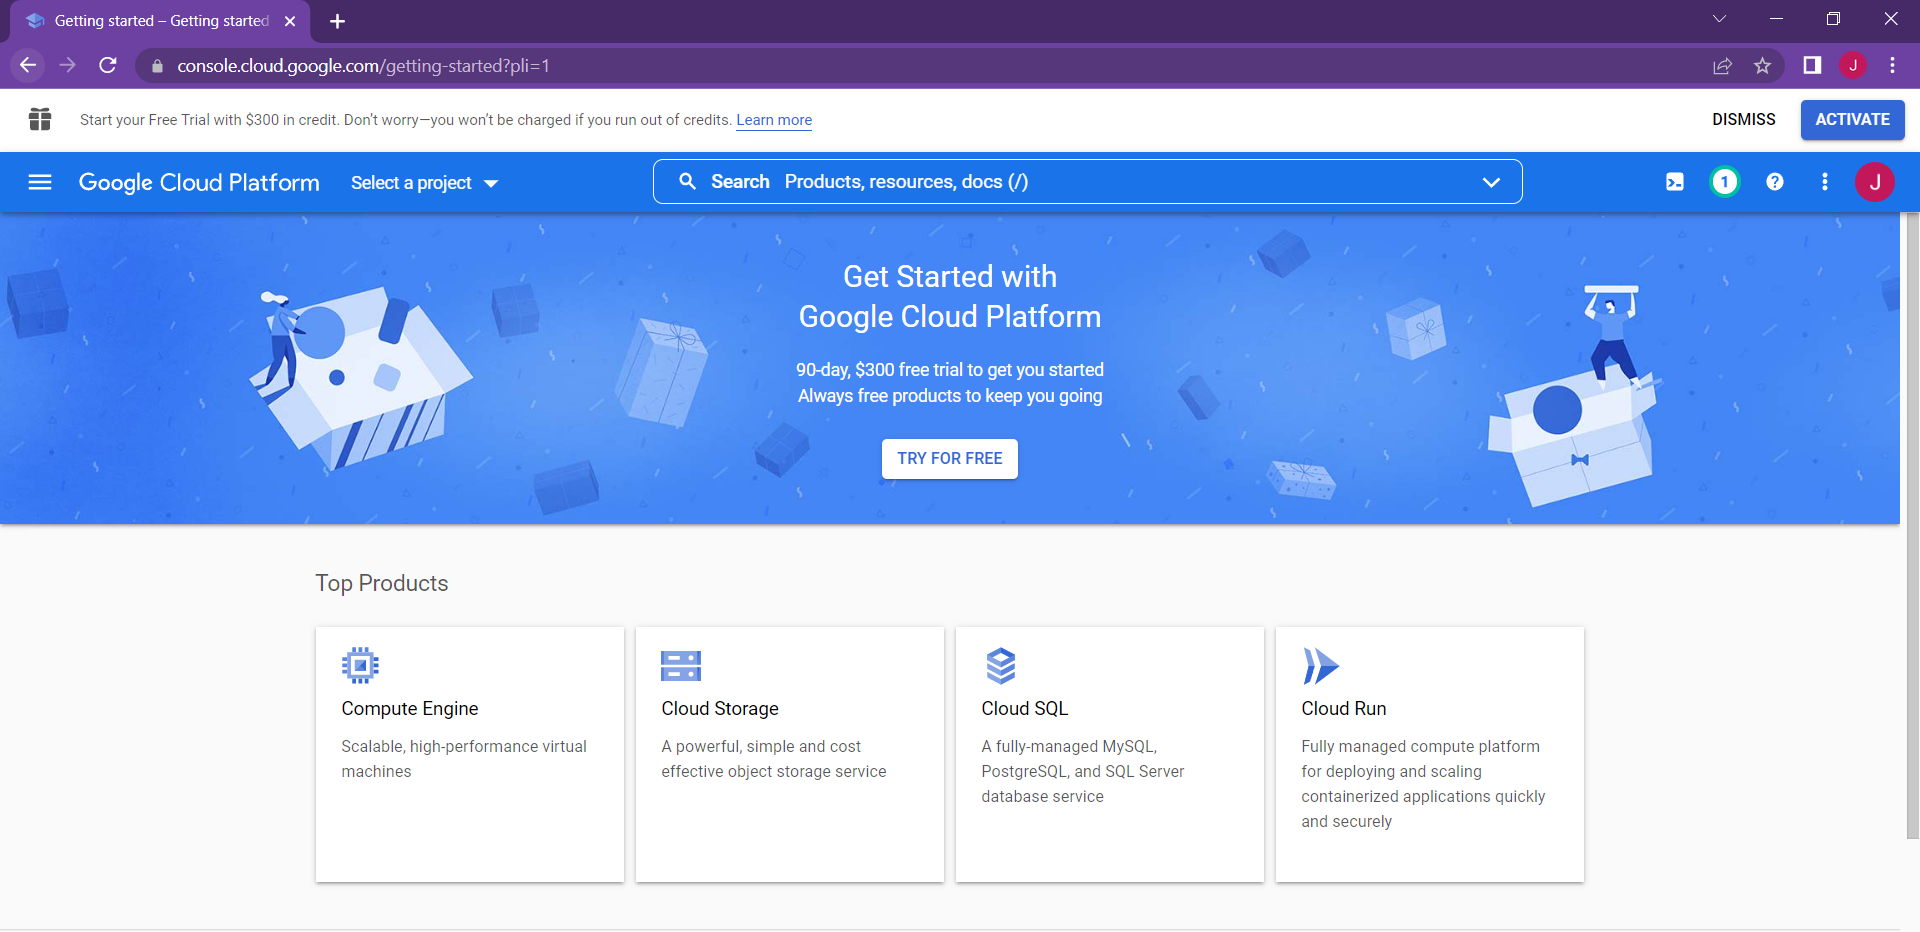
\includegraphics[scale=0.35]{Gambar/Google BigQuery HomePage.PNG}  
		\caption{Halaman Awal Google Cloud Project} 
		\label{fig:GCP_HP} 
	\end{figure}
	
	\item Memilih project kemudian \textit{"New Project"}
	\begin{figure}[H]
		\centering  
		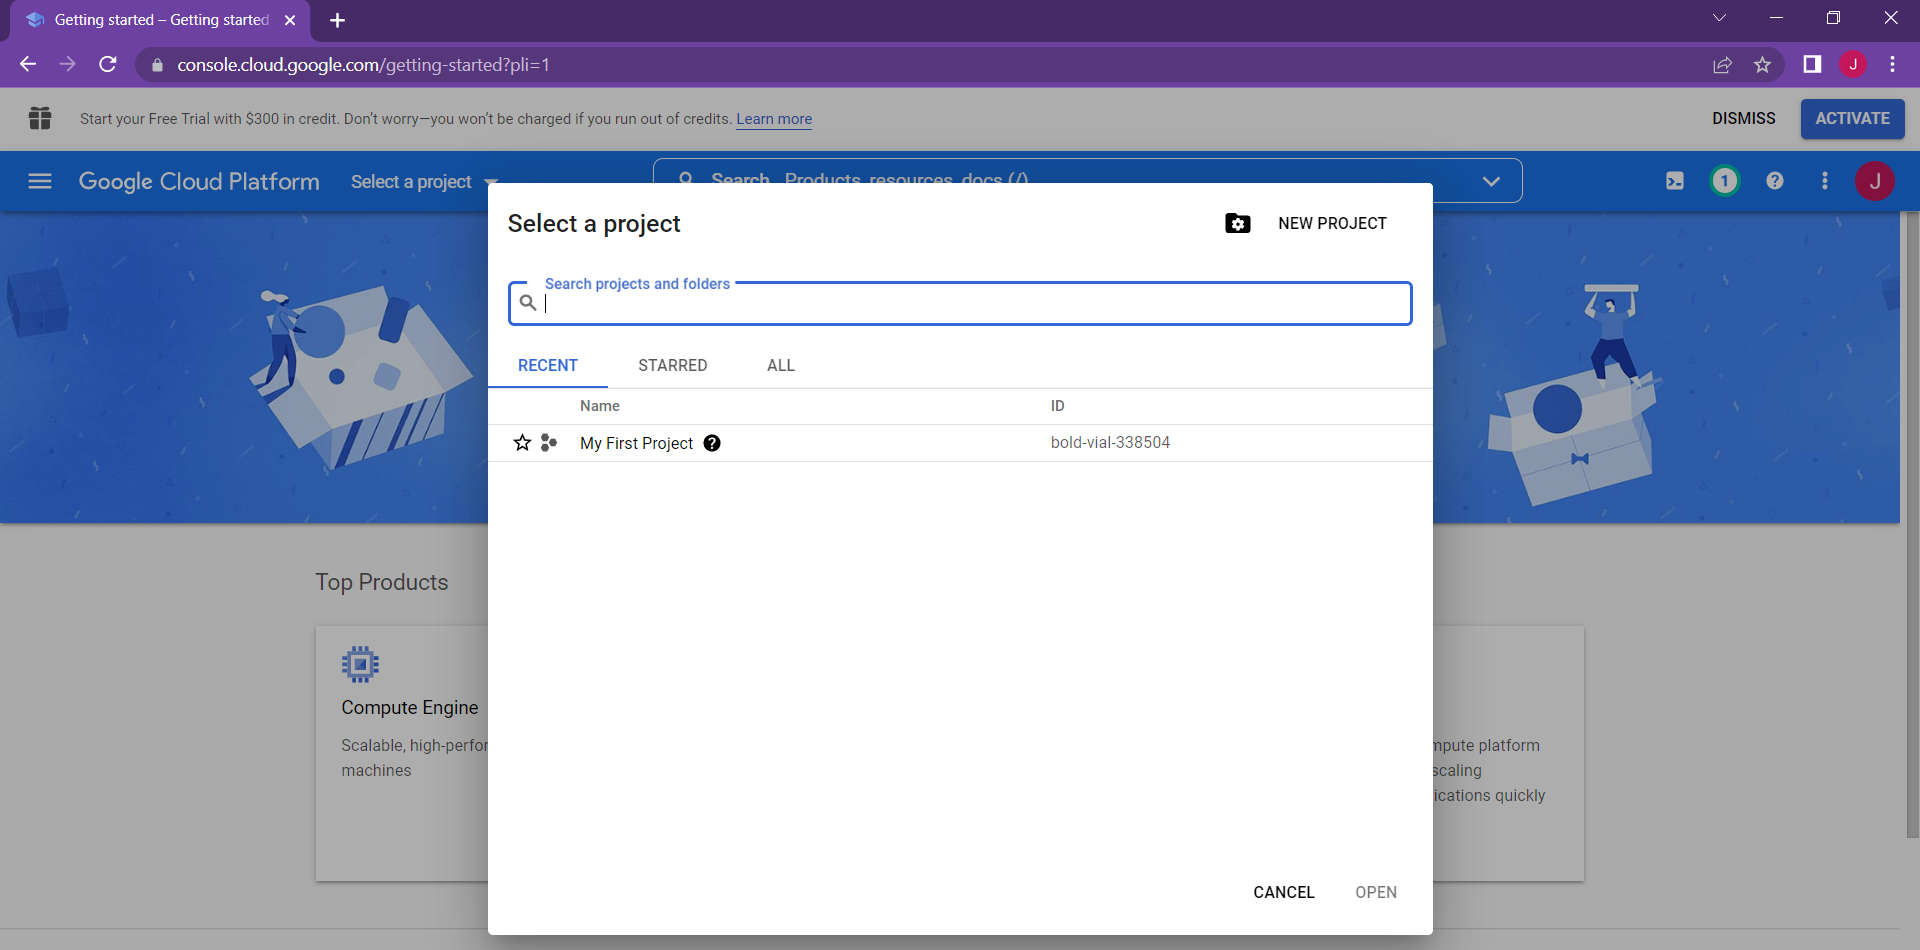
\includegraphics[scale=0.35]{Gambar/create_new_project.PNG}  
		\caption{Memilih \textit{Project}} 
		\label{fig:select_project} 
	\end{figure}
	
	\item Masukkan nama \textit{project} kemudian tekan tombol \textit{create}
	\begin{figure}[H]
		\centering  
		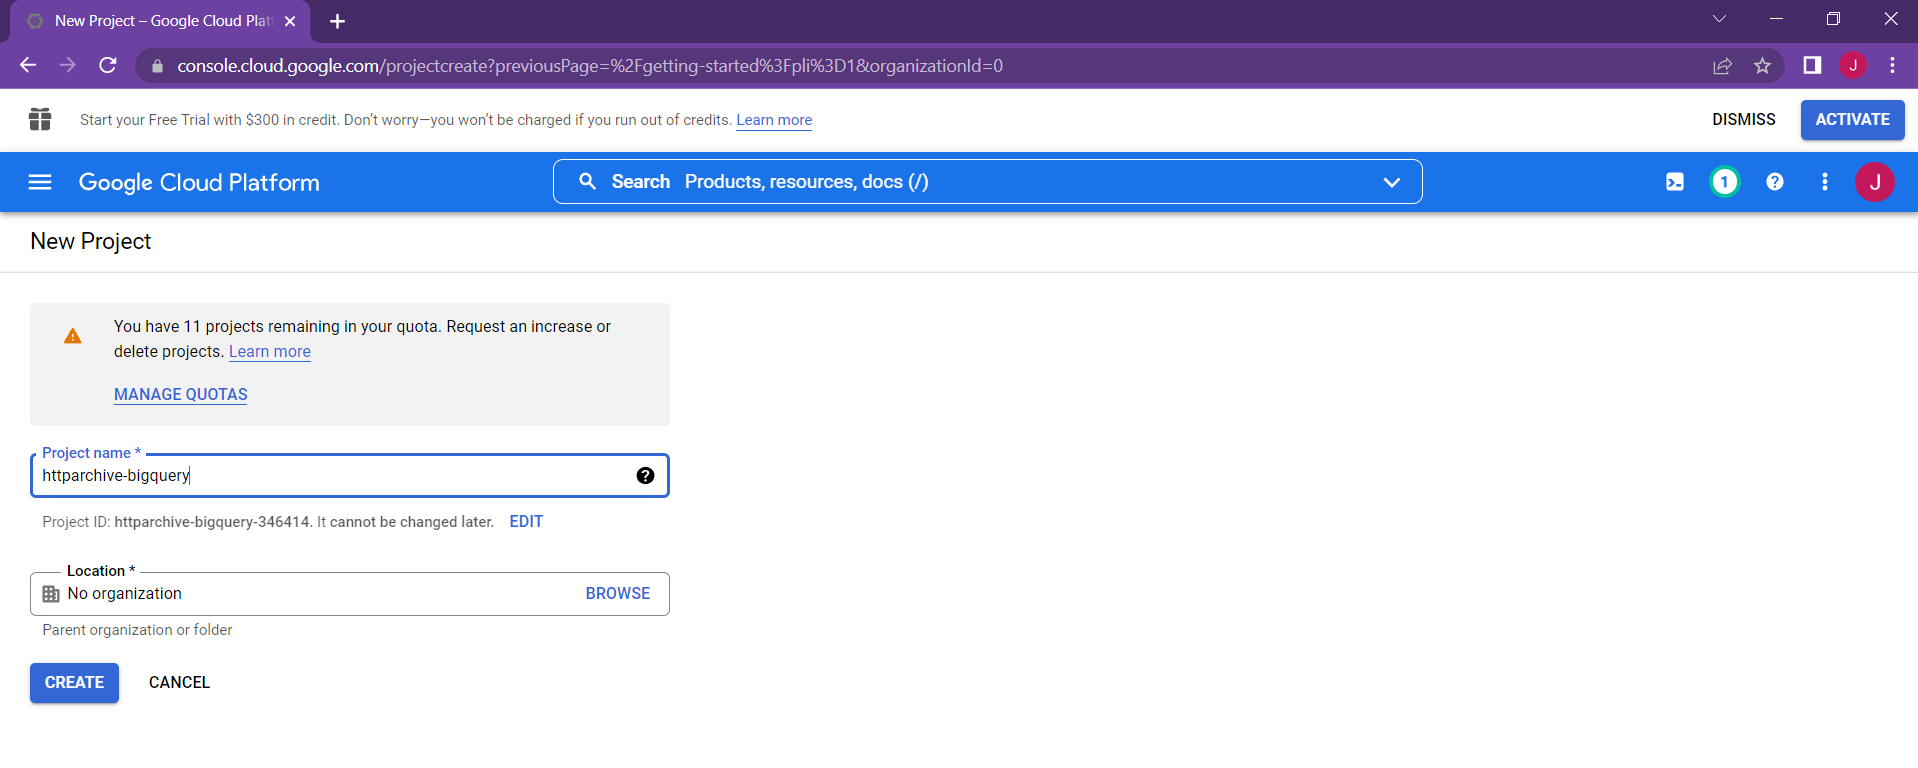
\includegraphics[scale=0.45]{Gambar/create_project.PNG}  
		\caption{Membuat \textit{Project}} 
		\label{fig:create_project} 
	\end{figure}
	
	\item Buka BigQuery \textit{console} 
	\begin{figure}[H]
		\centering  
		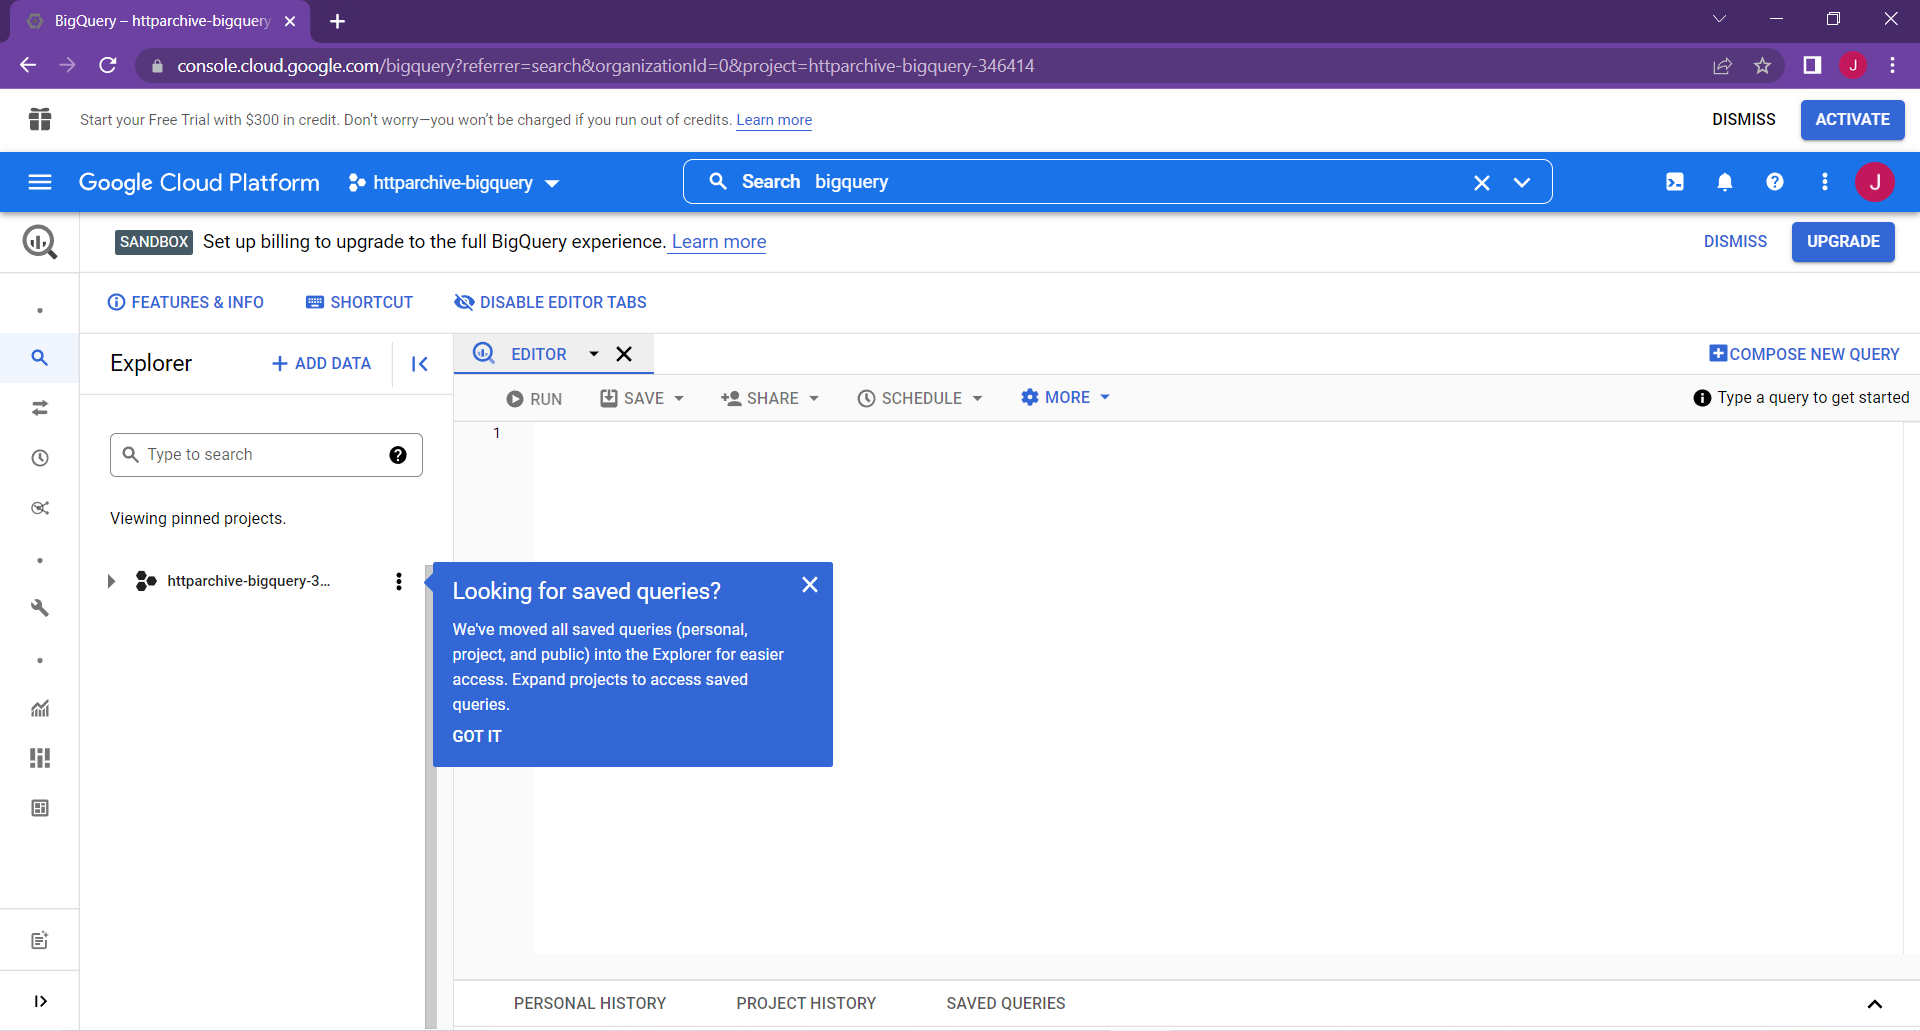
\includegraphics[scale=0.35]{Gambar/bq_workspace.PNG}  
		\caption{Membuka \textit{Console}} 
		\label{fig:open_console} 
	\end{figure}
	
	\item Untuk menambahkan tabel HTTP Archive pada \textit{project} didapatkan dari link \footnote{https://console.cloud.google.com/bigquery?p=httparchive}
	
	
	\item Data HTTP Archive dapat dilihat pada dashboard BigQuery.
	\begin{figure}[H]
		\centering  
		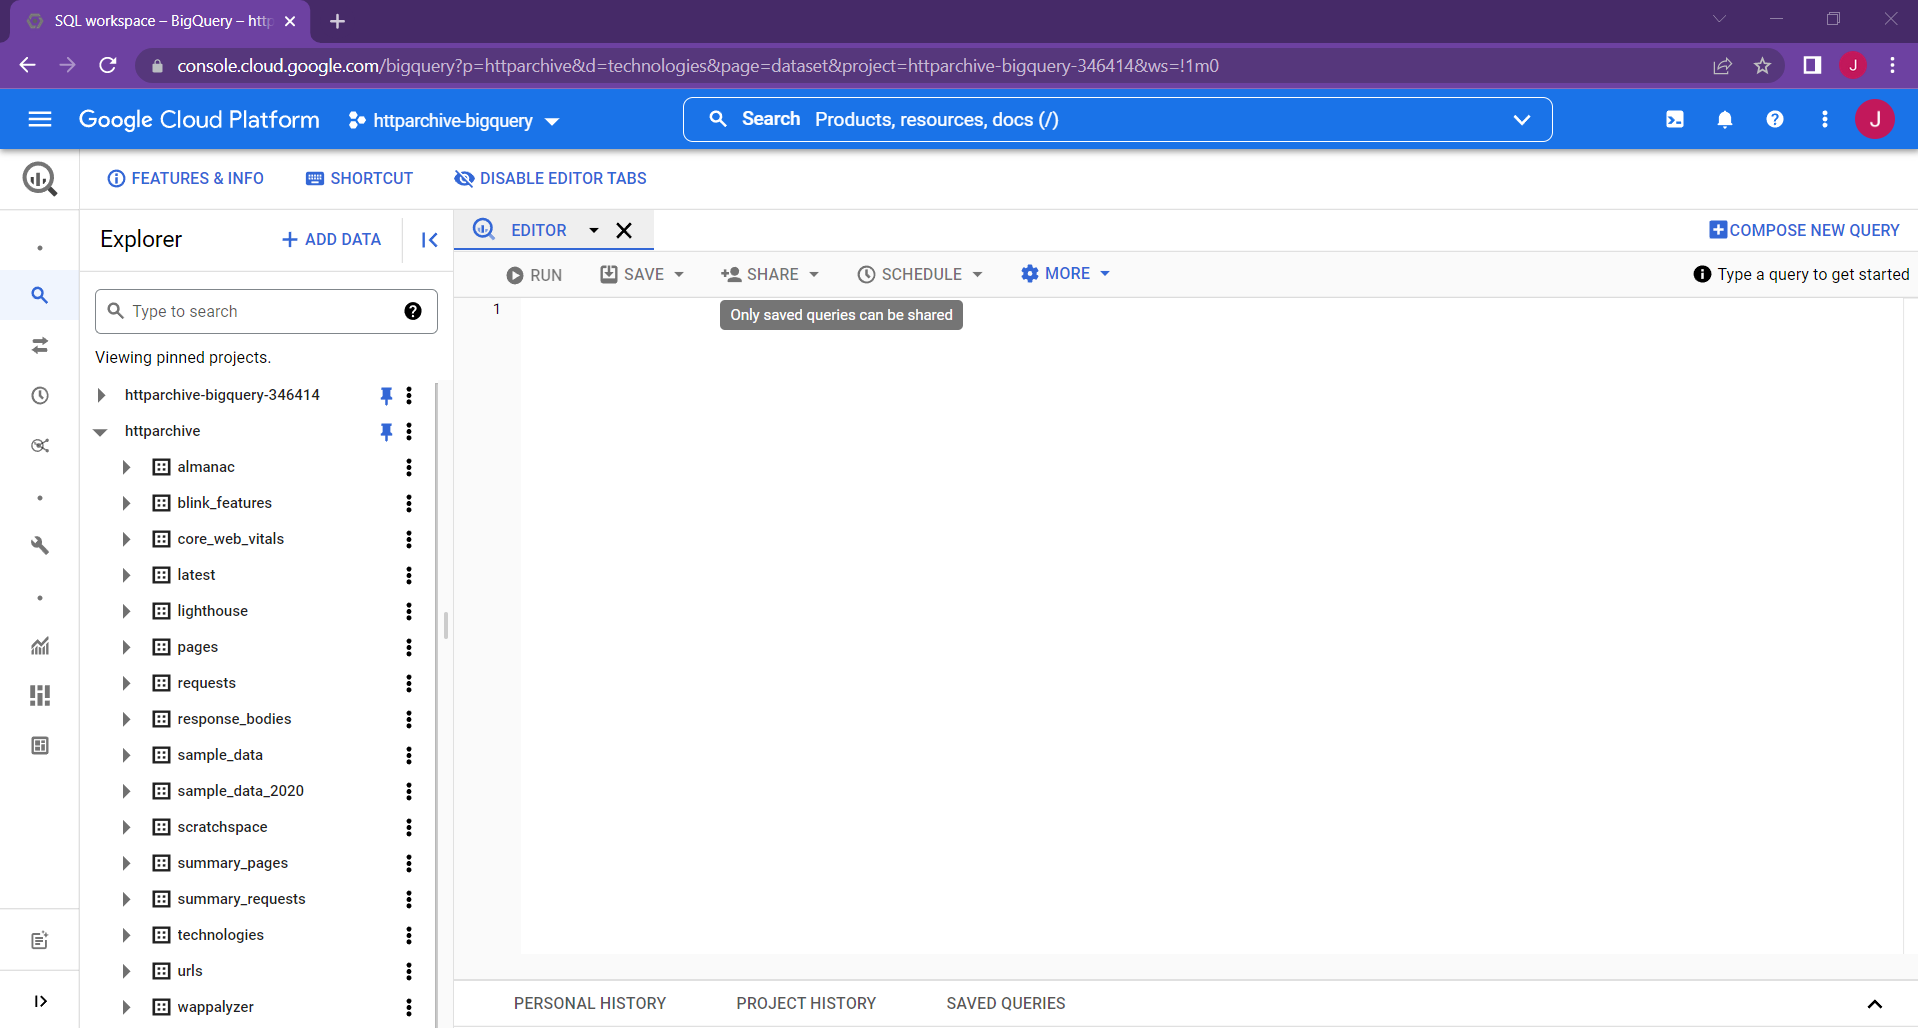
\includegraphics[scale=0.35]{Gambar/BG-Dashboard.PNG}  
		\caption{Data Terlihat Pada Dashboard} 
		\label{fig:BQ-Dashboard} 
	\end{figure}
\end{enumerate}

Di dalam BigQuery, terdapat salah satu fitur yang digunakan yaitu membuat \textit{dataset} baru. \textit{Dataset} bisa saja diambil dari \textit{public dataset} maupun membuat sendiri \textit{dataset} tersbut. \textit{Dataset} berisi tabel-tabel yang dianalisis. Tabel-tabel tersebut dapat dibuat secara manual maupun di-\textit{upload}.

Berikut ini langkah-langkah dalam pembuatan dataset dan tabel:
\begin{enumerate}
	\item Membuka Google Cloud Project Page\footnote{https://console.cloud.google.com/getting-started}. Halaman yang ditampilkan dapat dilihat pada gambar \ref{fig:GCP}
	\begin{figure}[H]
		\centering  
		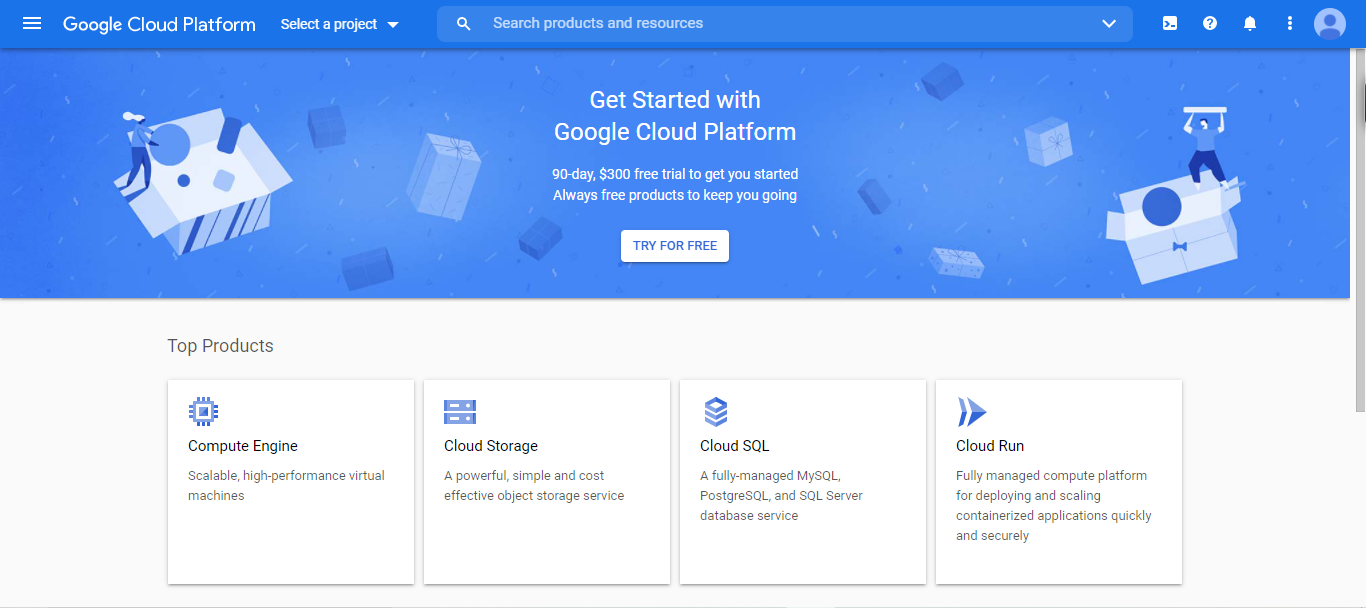
\includegraphics[scale=0.45]{Gambar/open_GCP.PNG}  
		\caption{Google Cloud Project Page} 
		\label{fig:GCP} 
	\end{figure}
	\item Membuat atau memilih \textit{project} yang dikerjakan. Halaman yang ditampilkan dapat dilihat pada gambar \ref{fig:create_or_open}
	\begin{figure}[H]
		\centering  
		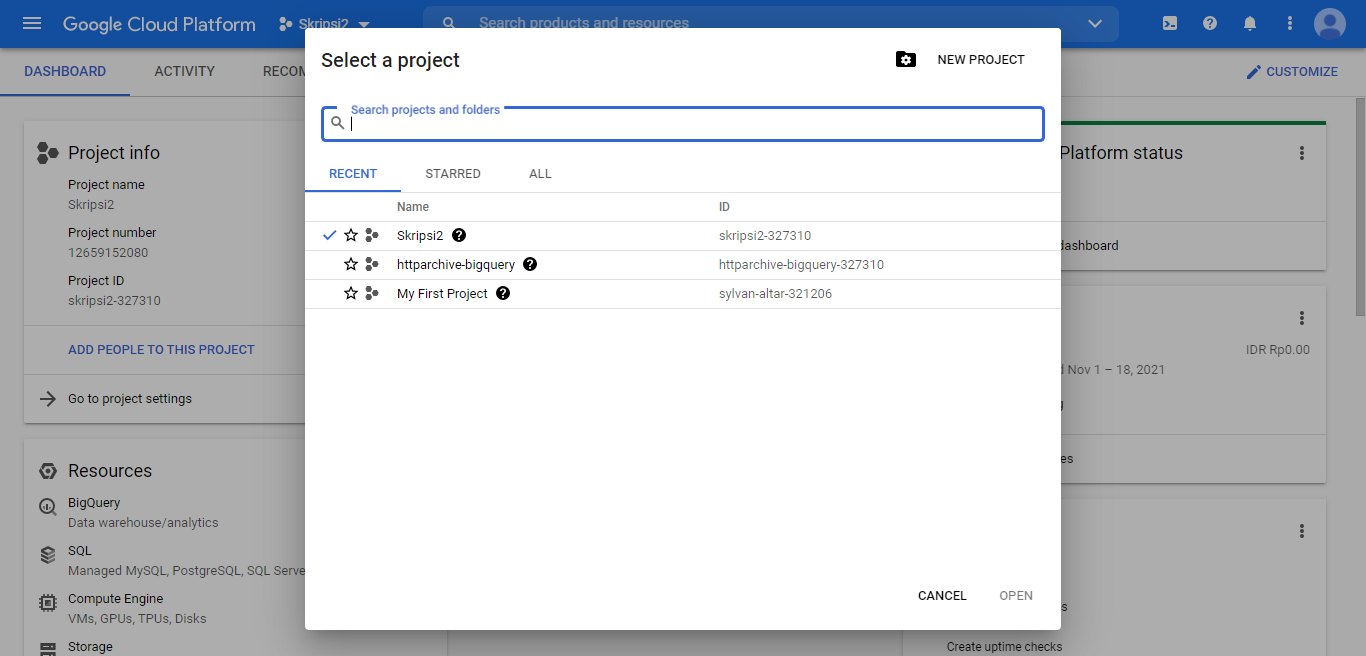
\includegraphics[scale=0.45]{Gambar/pilih_project.PNG}  
		\caption{Create atau Open Project} 
		\label{fig:create_or_open} 
	\end{figure}
	\item Membuka \textit{console} kemudian memilih BigQuery. Halaman yang ditampilkan dapat dilihat pada gambar \ref{fig:BQ}
	\begin{figure}[H]
		\centering  
		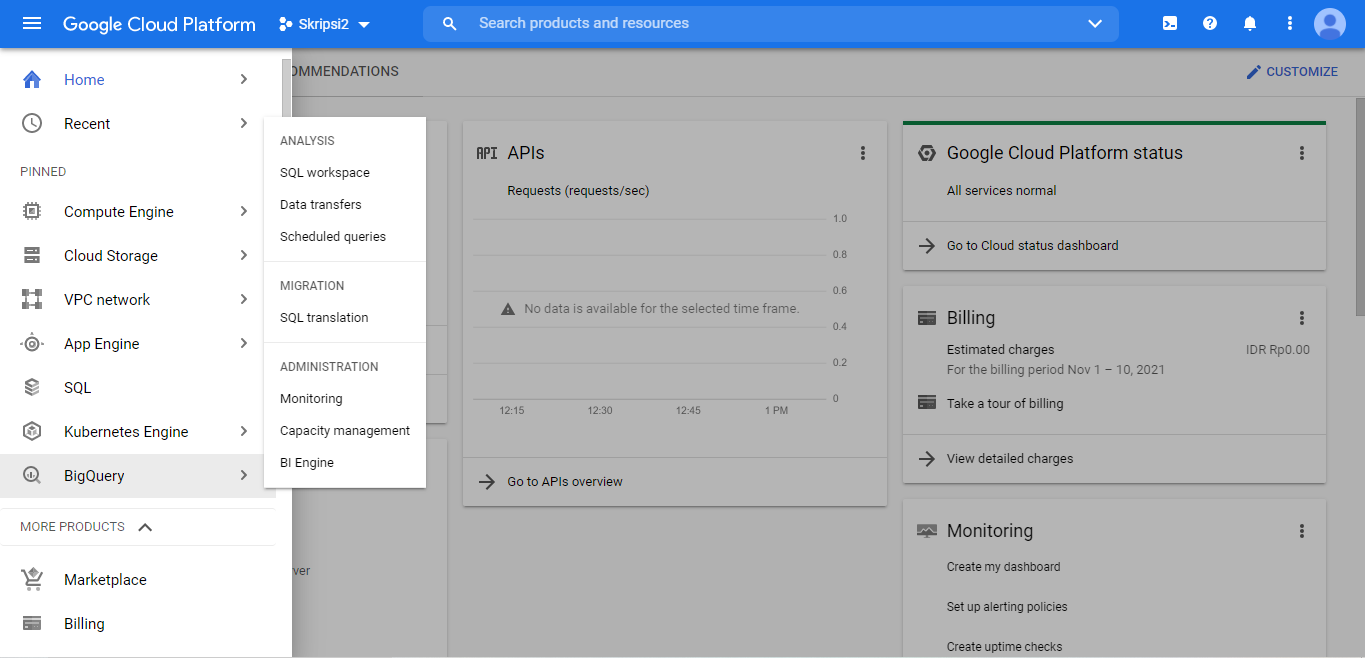
\includegraphics[scale=0.45]{Gambar/console_BigQuery.PNG}  
		\caption{Membuka BigQuery} 
		\label{fig:BQ} 
	\end{figure}
	\item Pada tab explorer terdapat project kemudian pengguna harus menekan tombol titik tiga dan piliih \textit{create} dataset. Halaman yang ditampilkan dapat dilihat pada gambar \ref{fig:create_dataset}
	\begin{figure}[H]
		\centering  
		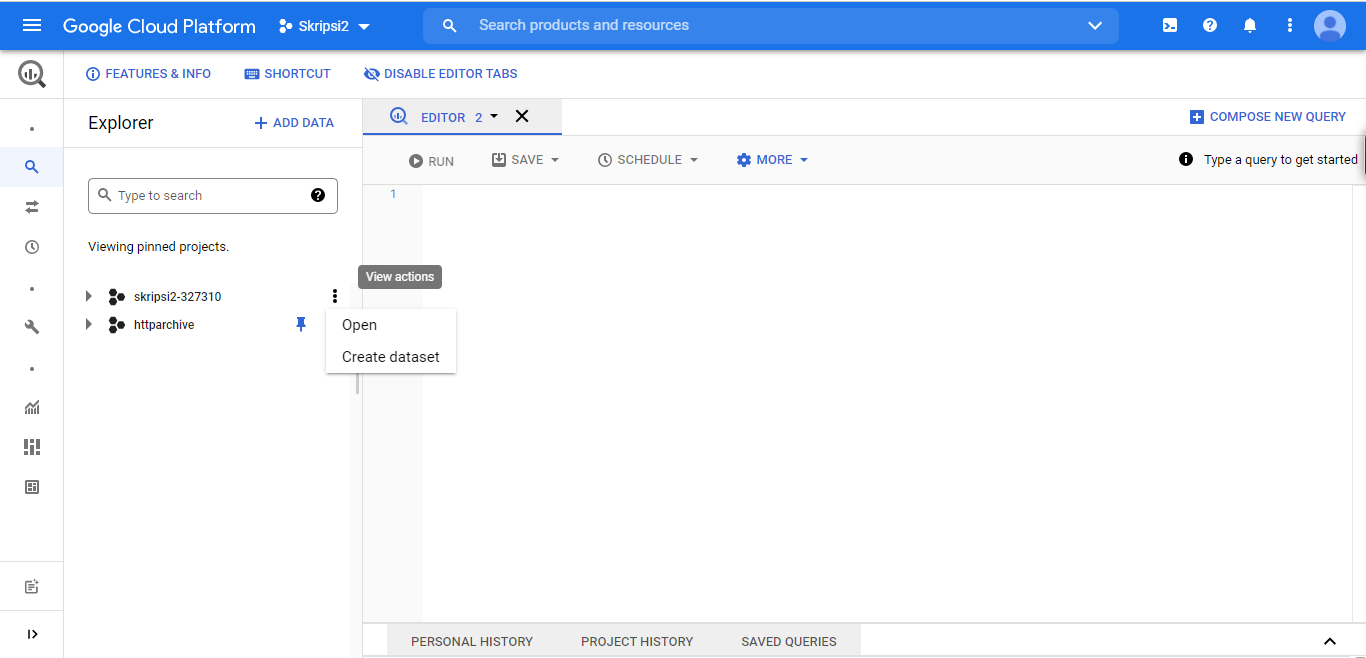
\includegraphics[scale=0.45]{Gambar/create_dataset.PNG}  
		\caption{Membuat Dataset Baru} 
		\label{fig:create_dataset} 
	\end{figure}
%	\item Buka dataset, kemudian pilih menu \textit{create table}. Halaman yang akan ditampilkan dapat dilihat pada gambar \ref{fig:create_table}
%	\begin{figure}[H]
%		\centering  
%		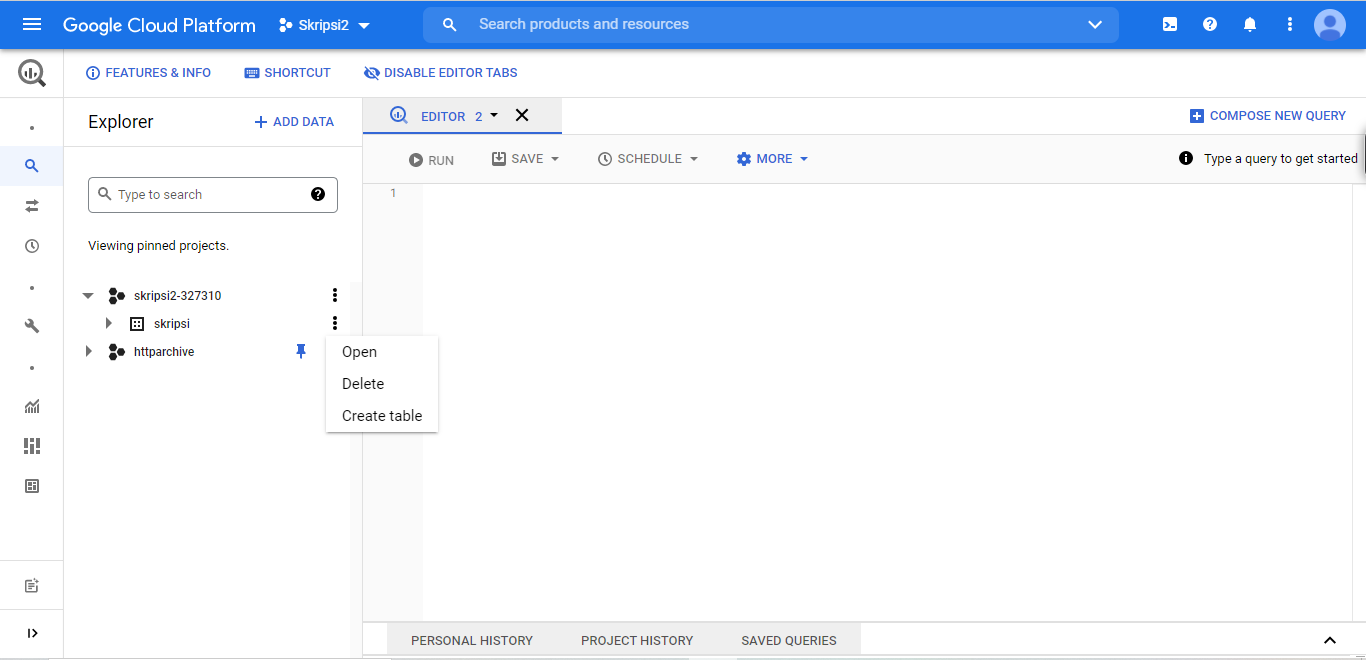
\includegraphics[scale=0.45]{Gambar/create_table.PNG}  
%		\caption{Membuat Tabel Baru} 
%		\label{fig:create_table} 
%	\end{figure}
\end{enumerate}

Skripsi ini membuat tabel baru agar tidak melakukan \textit{query} yang sama berulang. Tabel dapat dibuat dengan cara:
\begin{enumerate}
	\item Membuat query yang disimpan dalam tabel
	\begin{figure}[H]
	\centering  
	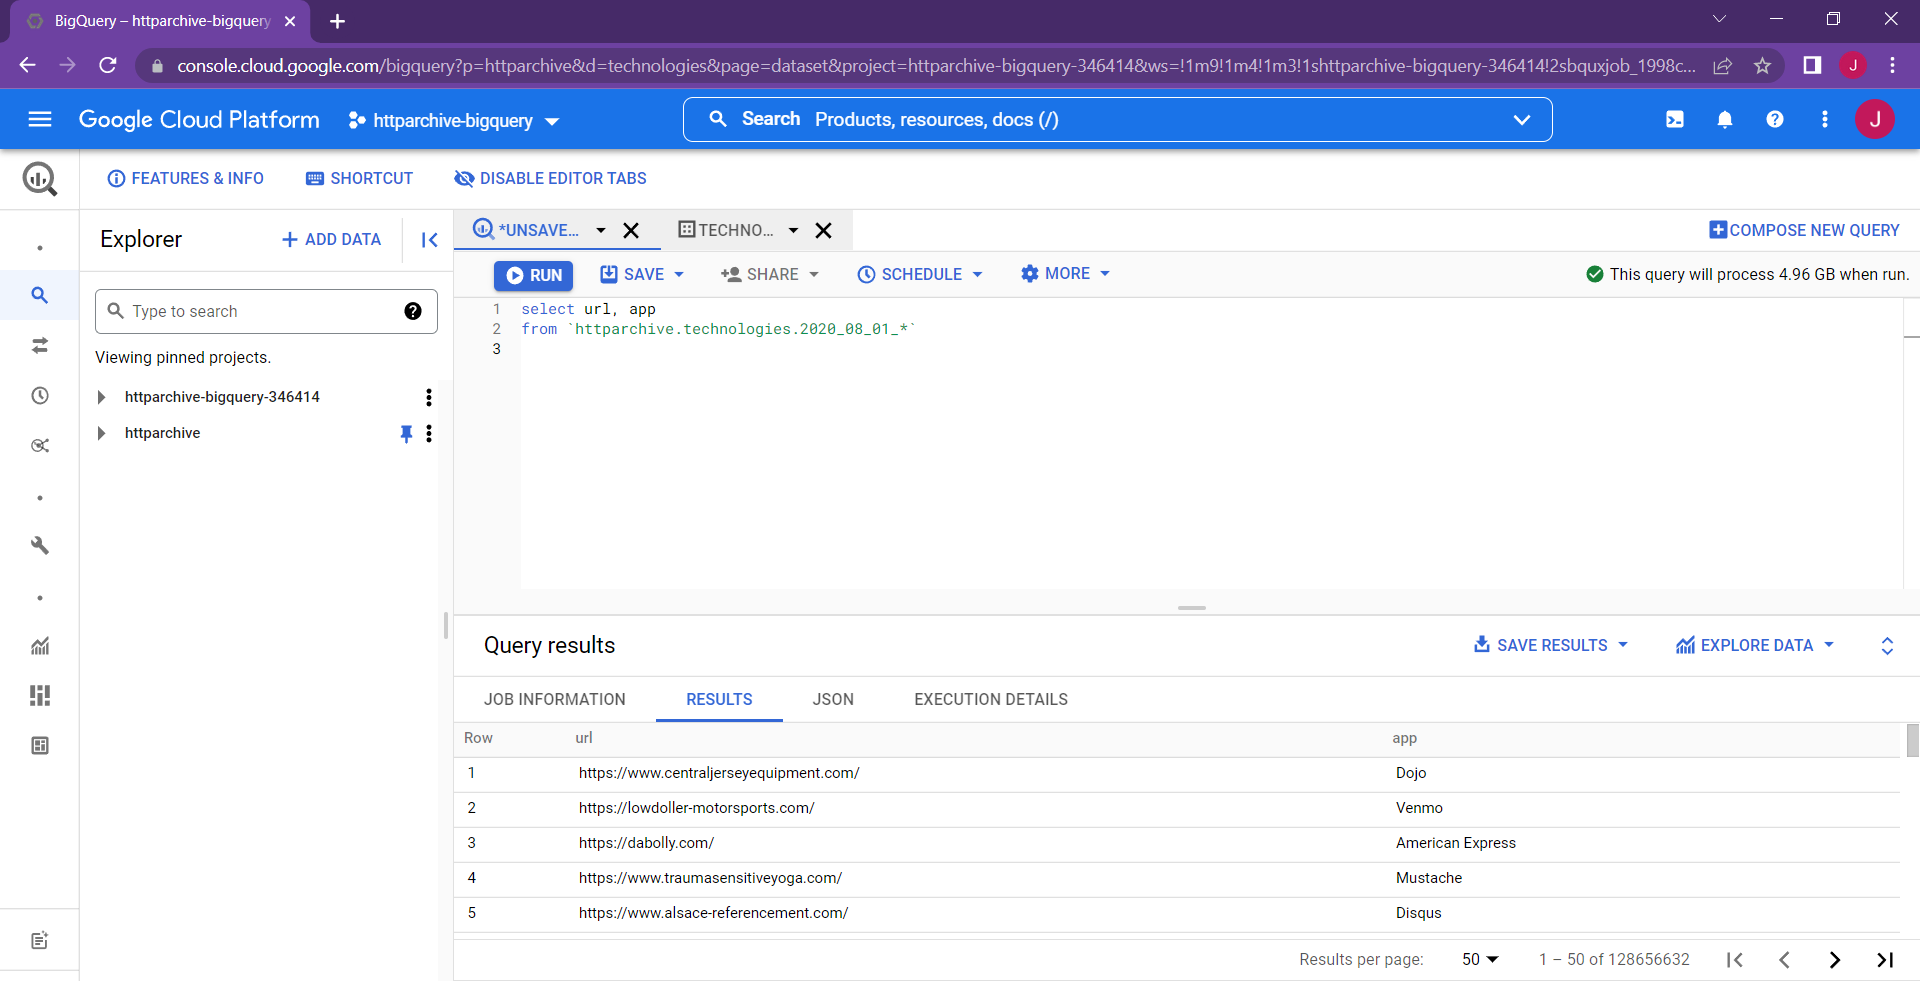
\includegraphics[scale=0.35]{Gambar/membuat query.PNG}  
	\caption{Membuat Tabel Baru} 
	\label{fig:create_table} 
\end{figure}
	\item Memilih \textit{save result} as BigQuery \textit{Table}
	\begin{figure}[H]
		\centering  
		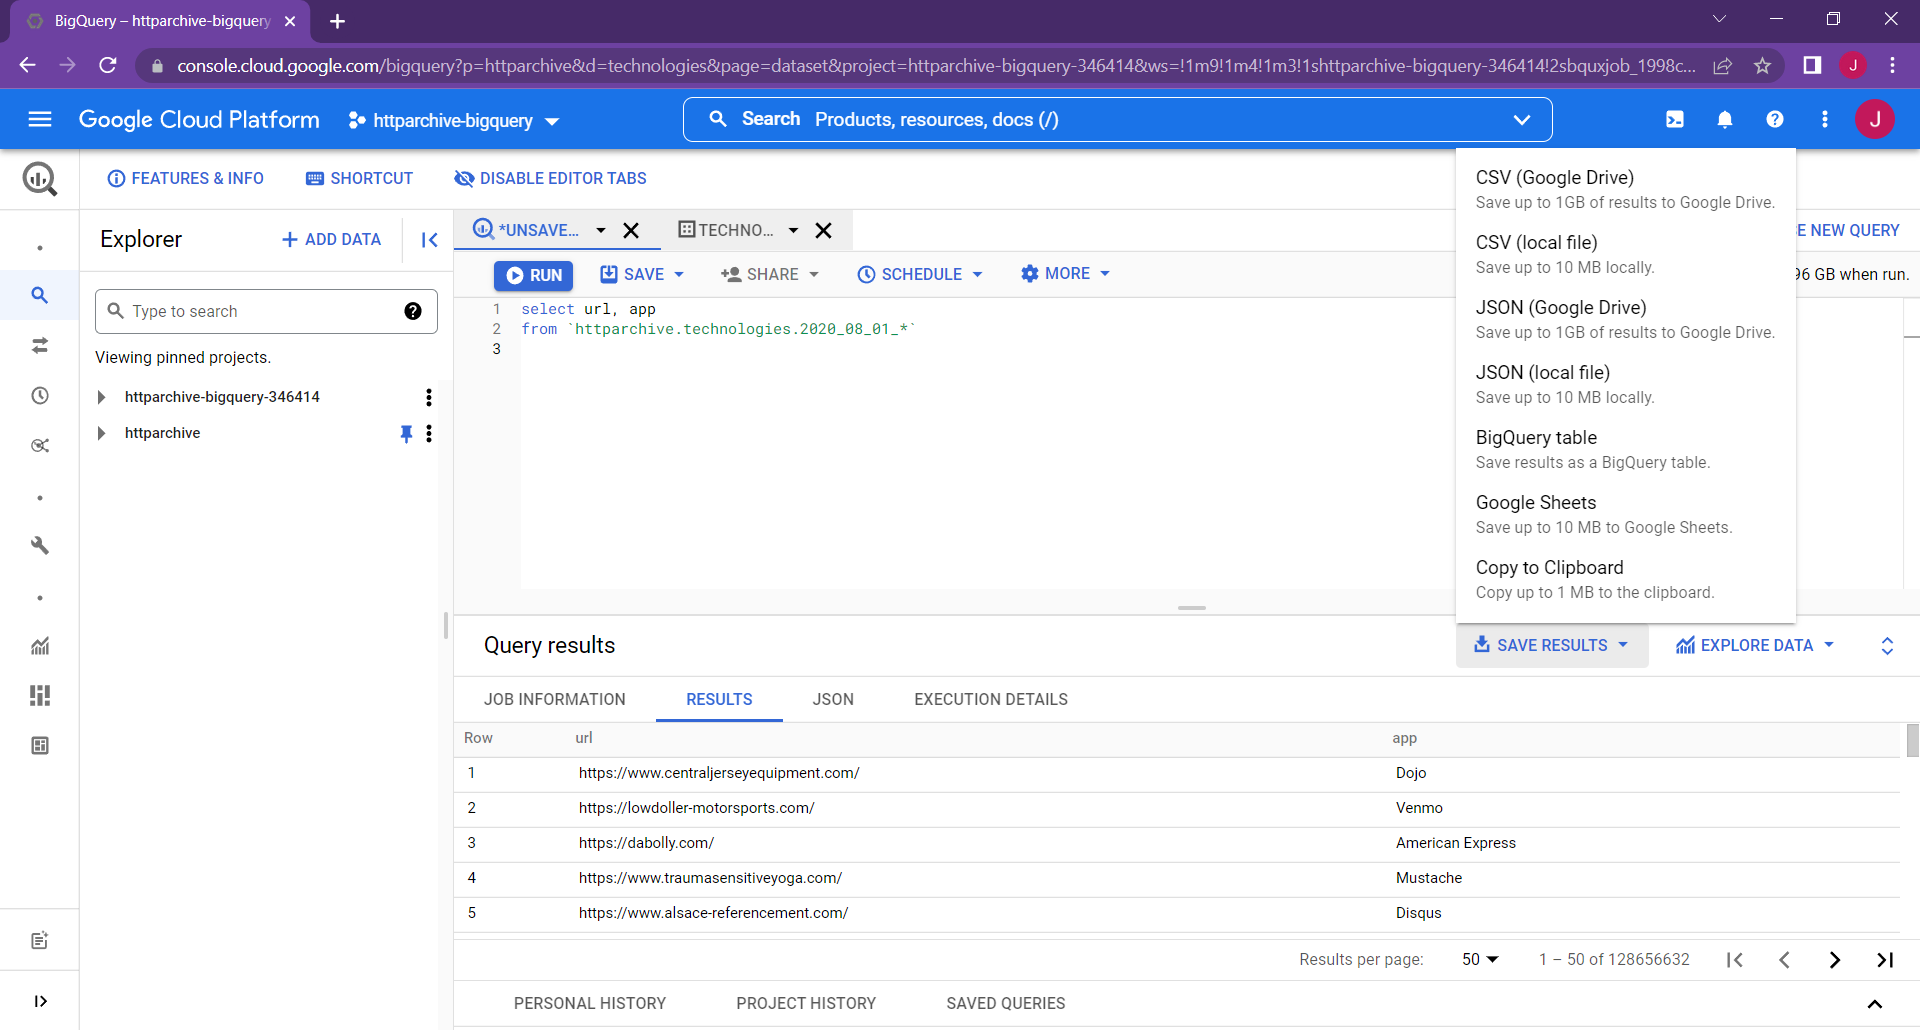
\includegraphics[scale=0.35]{Gambar/save bigquery table.PNG}  
		\caption{Memilih Save Result As BigQuery Table} 
		\label{fig:save_table}
	\end{figure}
	\item Memilih lokasi atau \textit{dataset} dan nama tabel untuk disimpan kemudian \textit{export}
	\begin{figure}[H]
		\centering  
		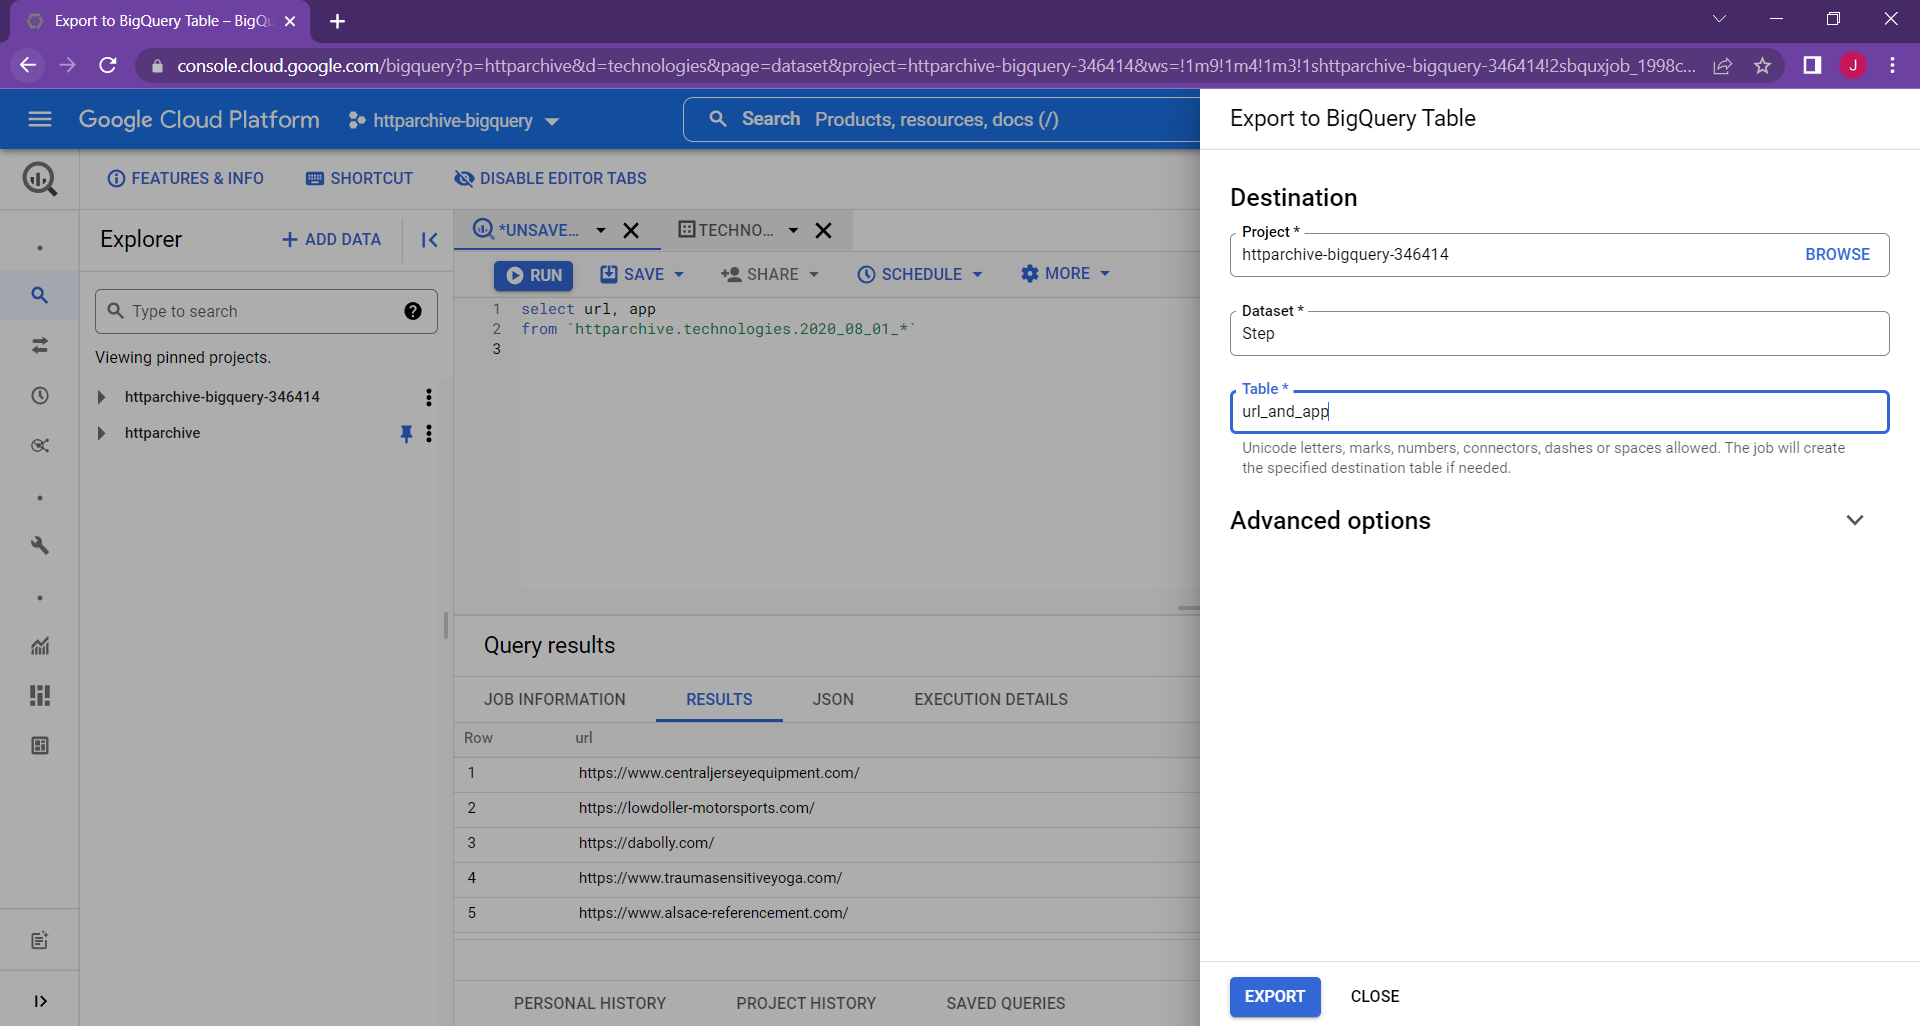
\includegraphics[scale=0.35]{Gambar/export table.PNG}  
		\caption{Export Table} 
		\label{fig:export_table}
	\end{figure}
	\item Lokasi tabel dapat dilihat pada \textit{dashboard}
		\begin{figure}[H]
		\centering  
		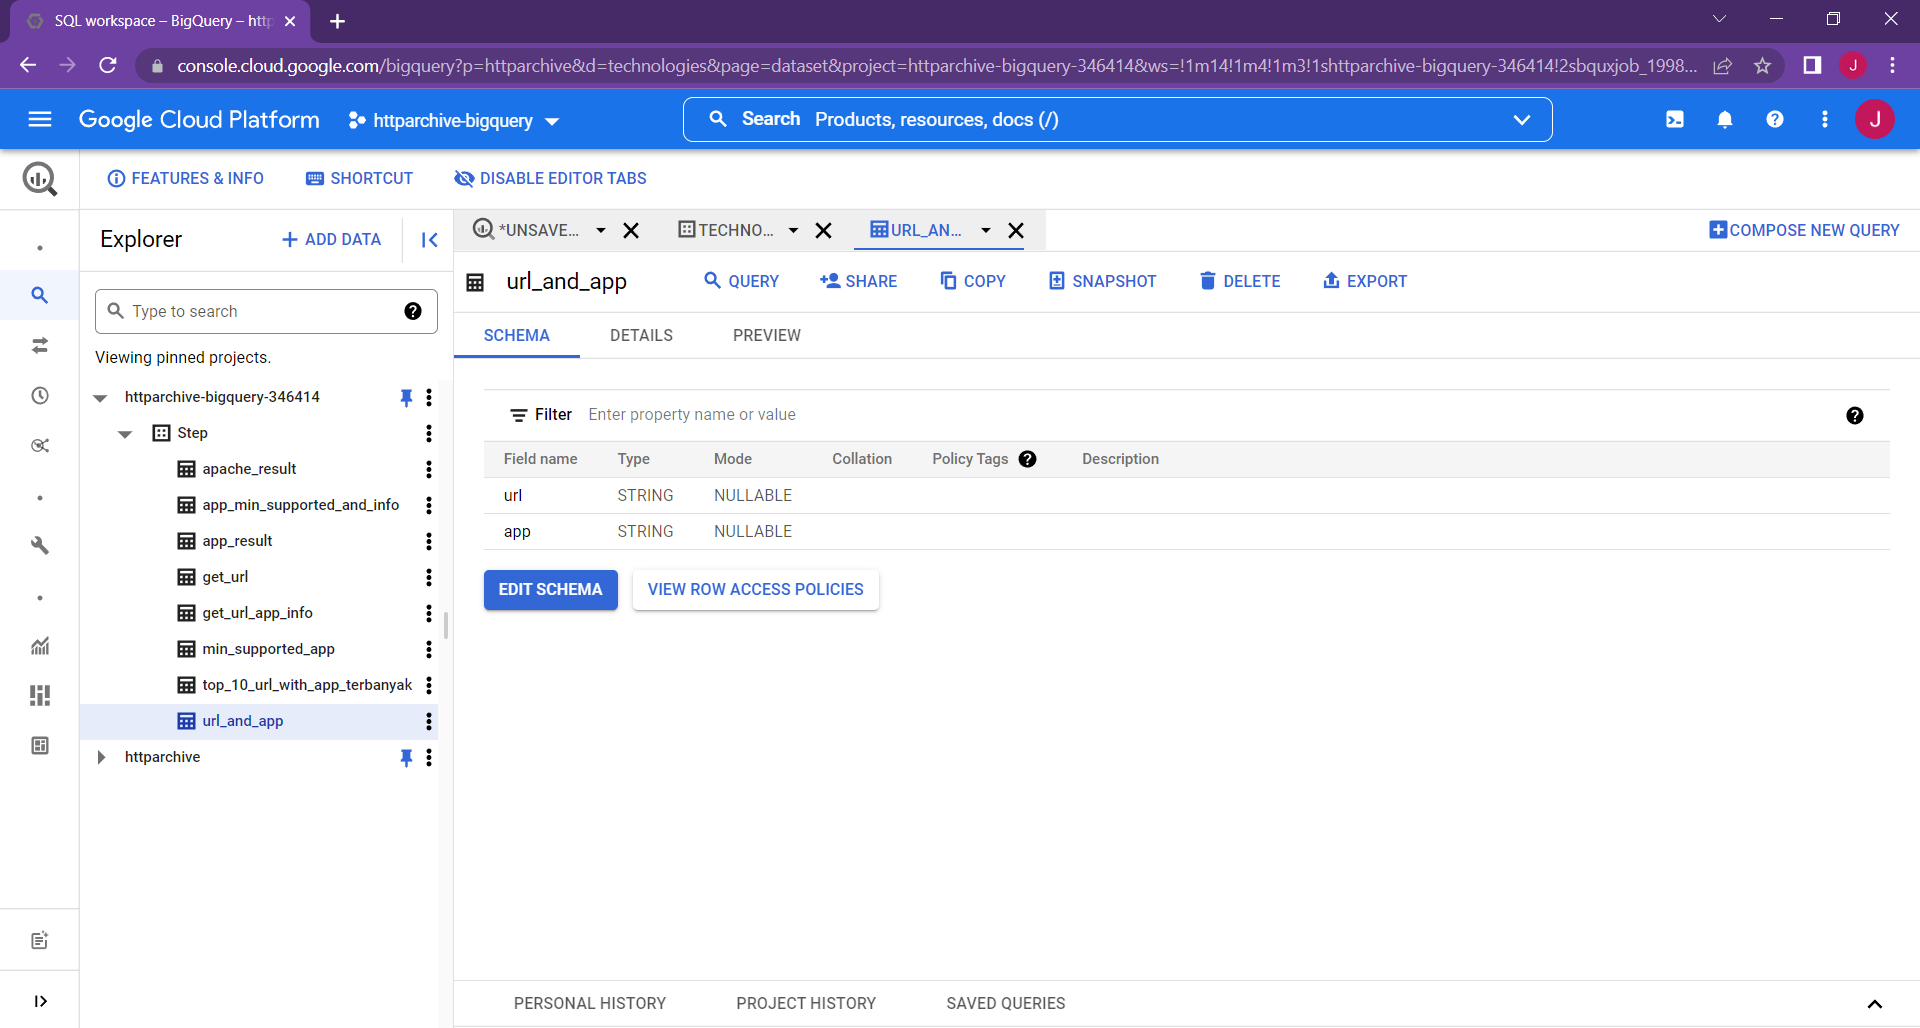
\includegraphics[scale=0.35]{Gambar/saved dashboard.PNG}  
		\caption{Dashboard Table} 
		\label{fig:lokasi_table}
	\end{figure}
\end{enumerate}

Selain itu, \textit{table} dapat dibuat dengan meng-\textit{upload} table dari CSV atau JSON. Tabel dapat dibuat dengan cara:
\begin{enumerate}
	\item Pilih titik tiga pada salah satu dataset dan pilih \textit{create table} yang dapat dilihat pada gambar\ref{upload1}.
	\begin{figure}[H]
		\centering  
		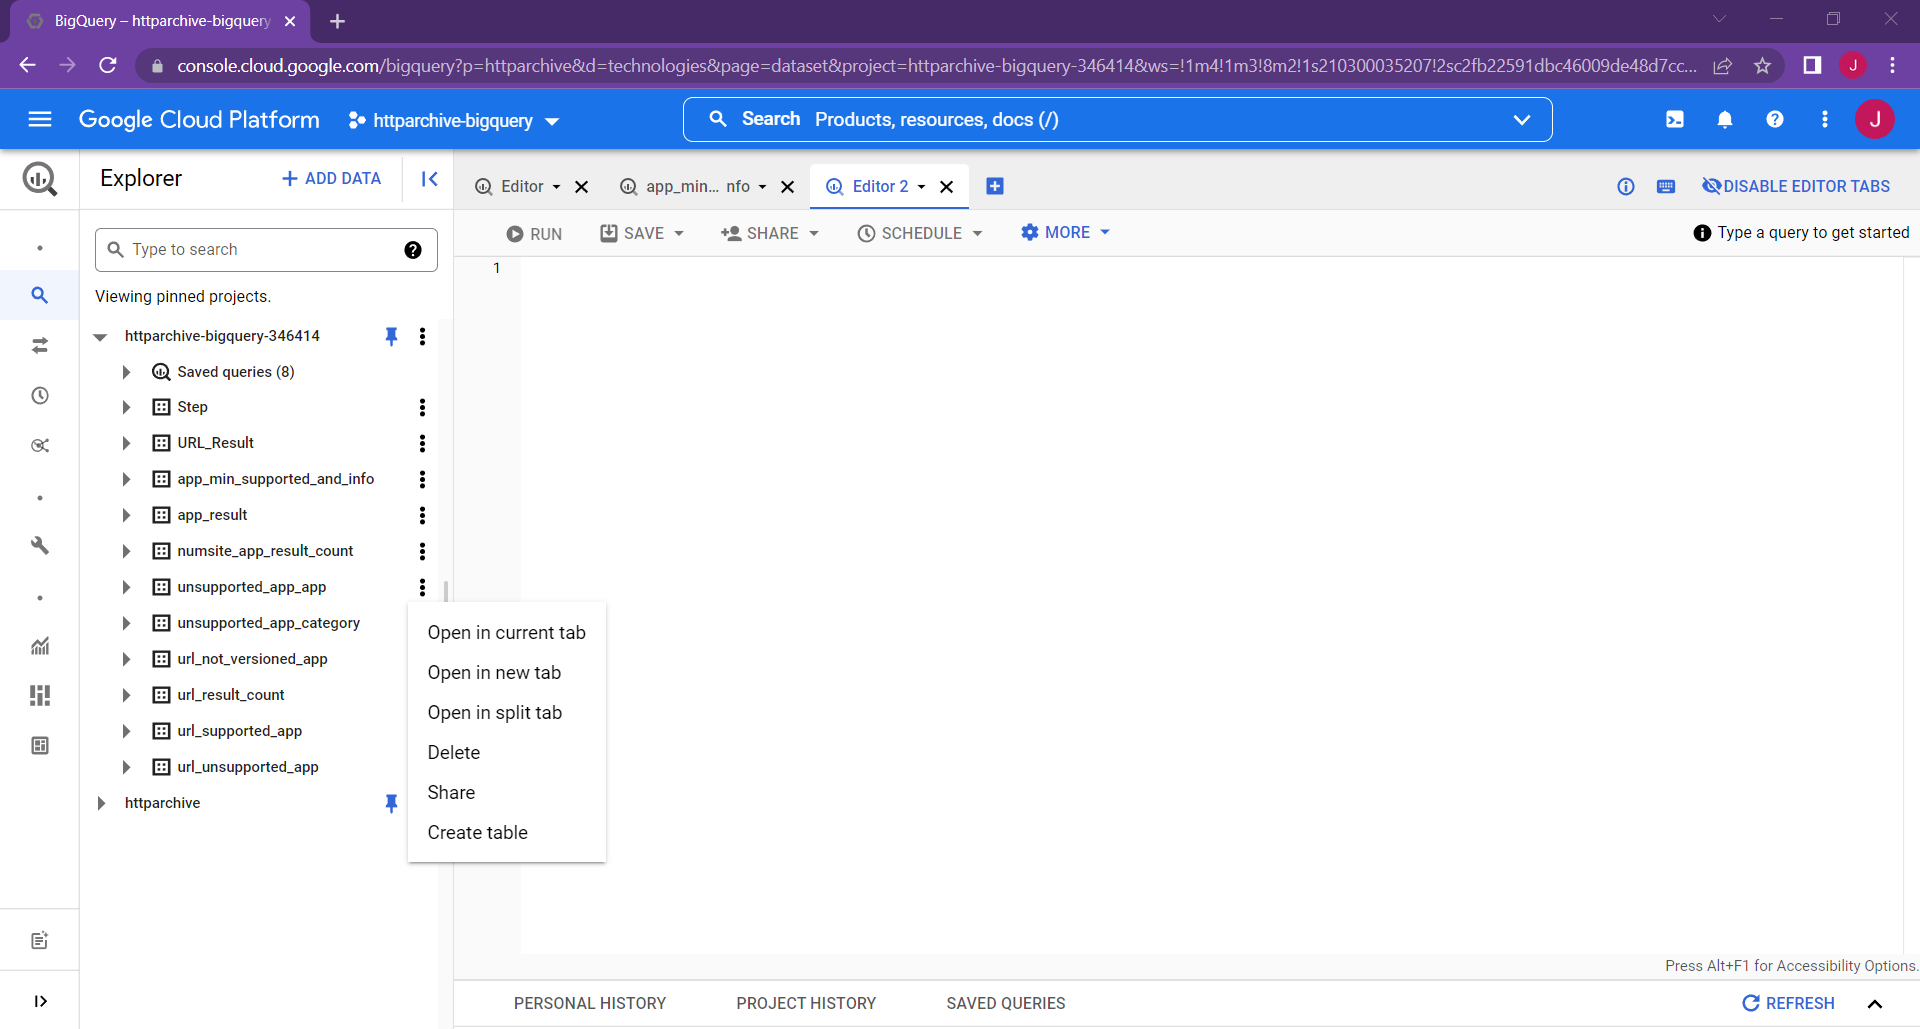
\includegraphics[scale=0.35]{Gambar/upload_step_1.png}  
		\caption{Create Table} 
		\label{fig:upload1}
	\end{figure}

	\item Kemudian pilih \textit{upload} pada \textit{field} \textit{create table from} yang dapat dilihat pada gambar\ref{fig:upload2}
	\begin{figure}[H]
		\centering  
		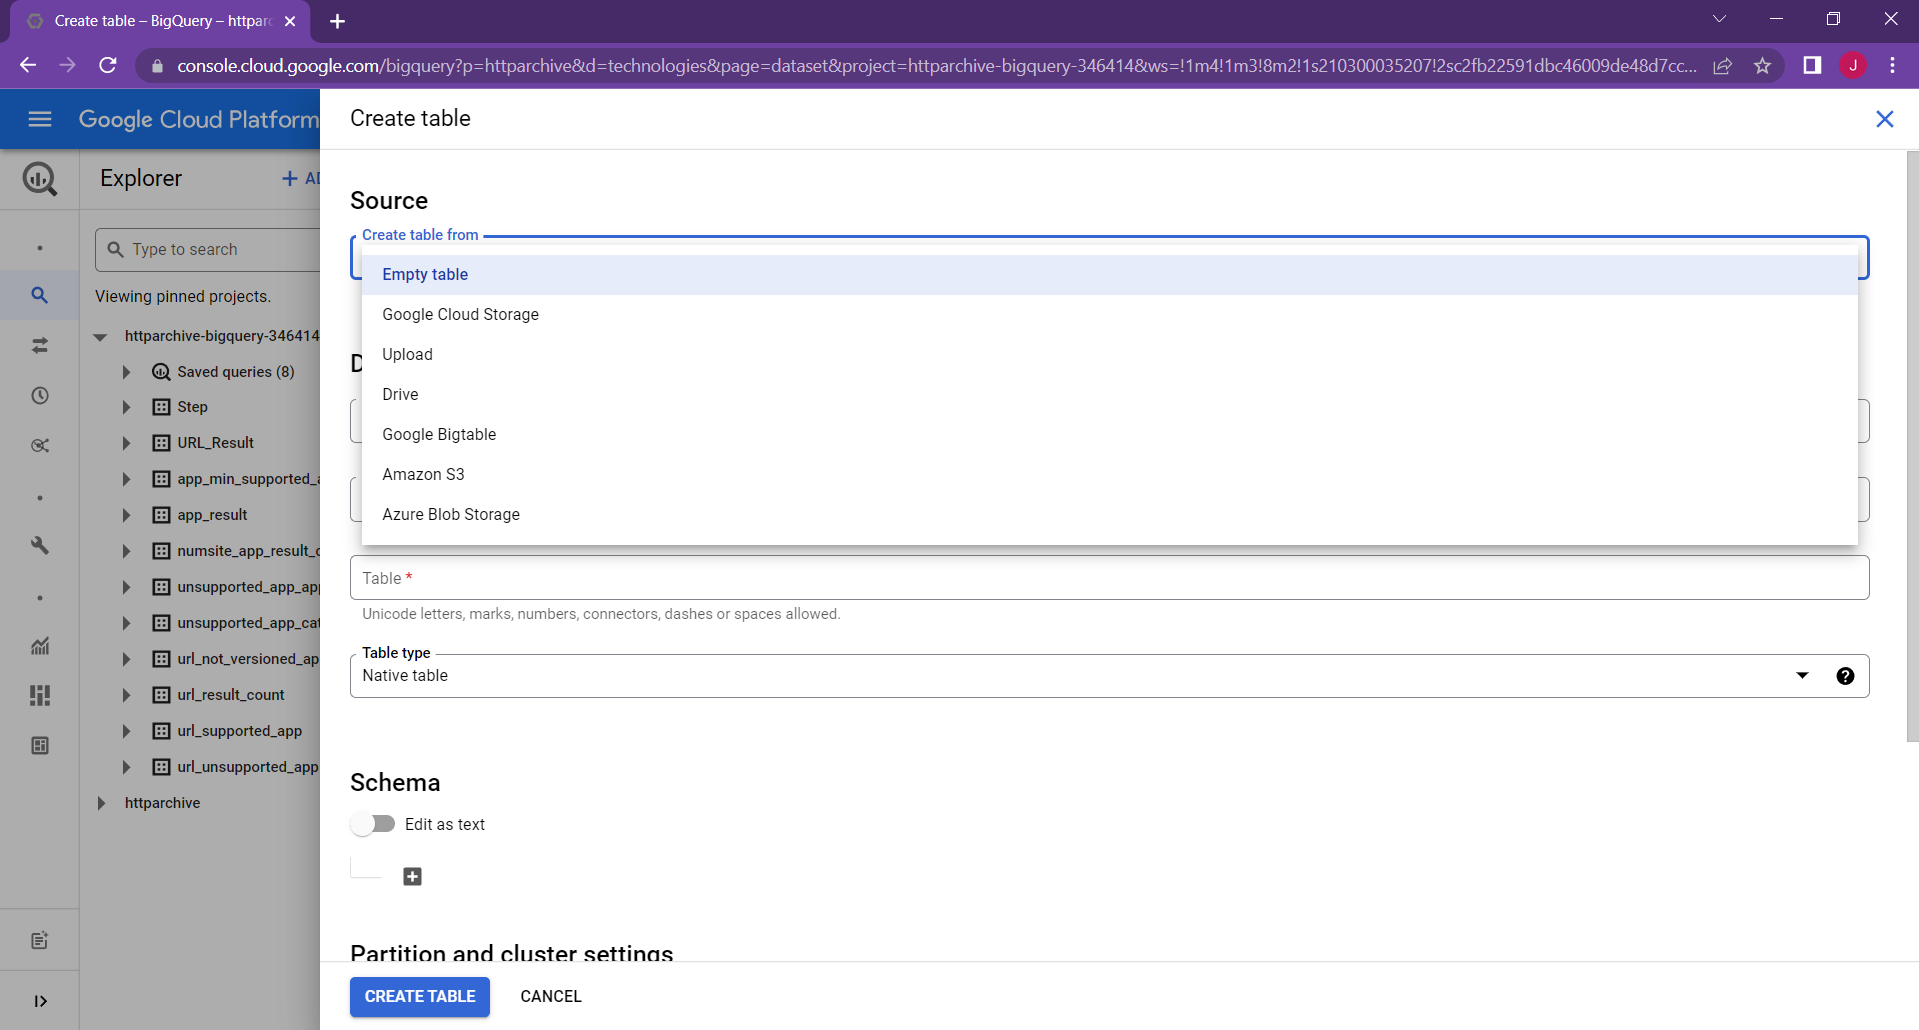
\includegraphics[scale=0.35]{Gambar/upload_step_2.png}  
		\caption{Pilih Upload} 
		\label{fig:upload2}
	\end{figure}

	\item Pilih lokasi \textit{file}, pilih format, dan nama tabel \textit{file} yang dapat dilihat pada gambar\ref{fig:upload3}
	\begin{figure}[H]
		\centering  
		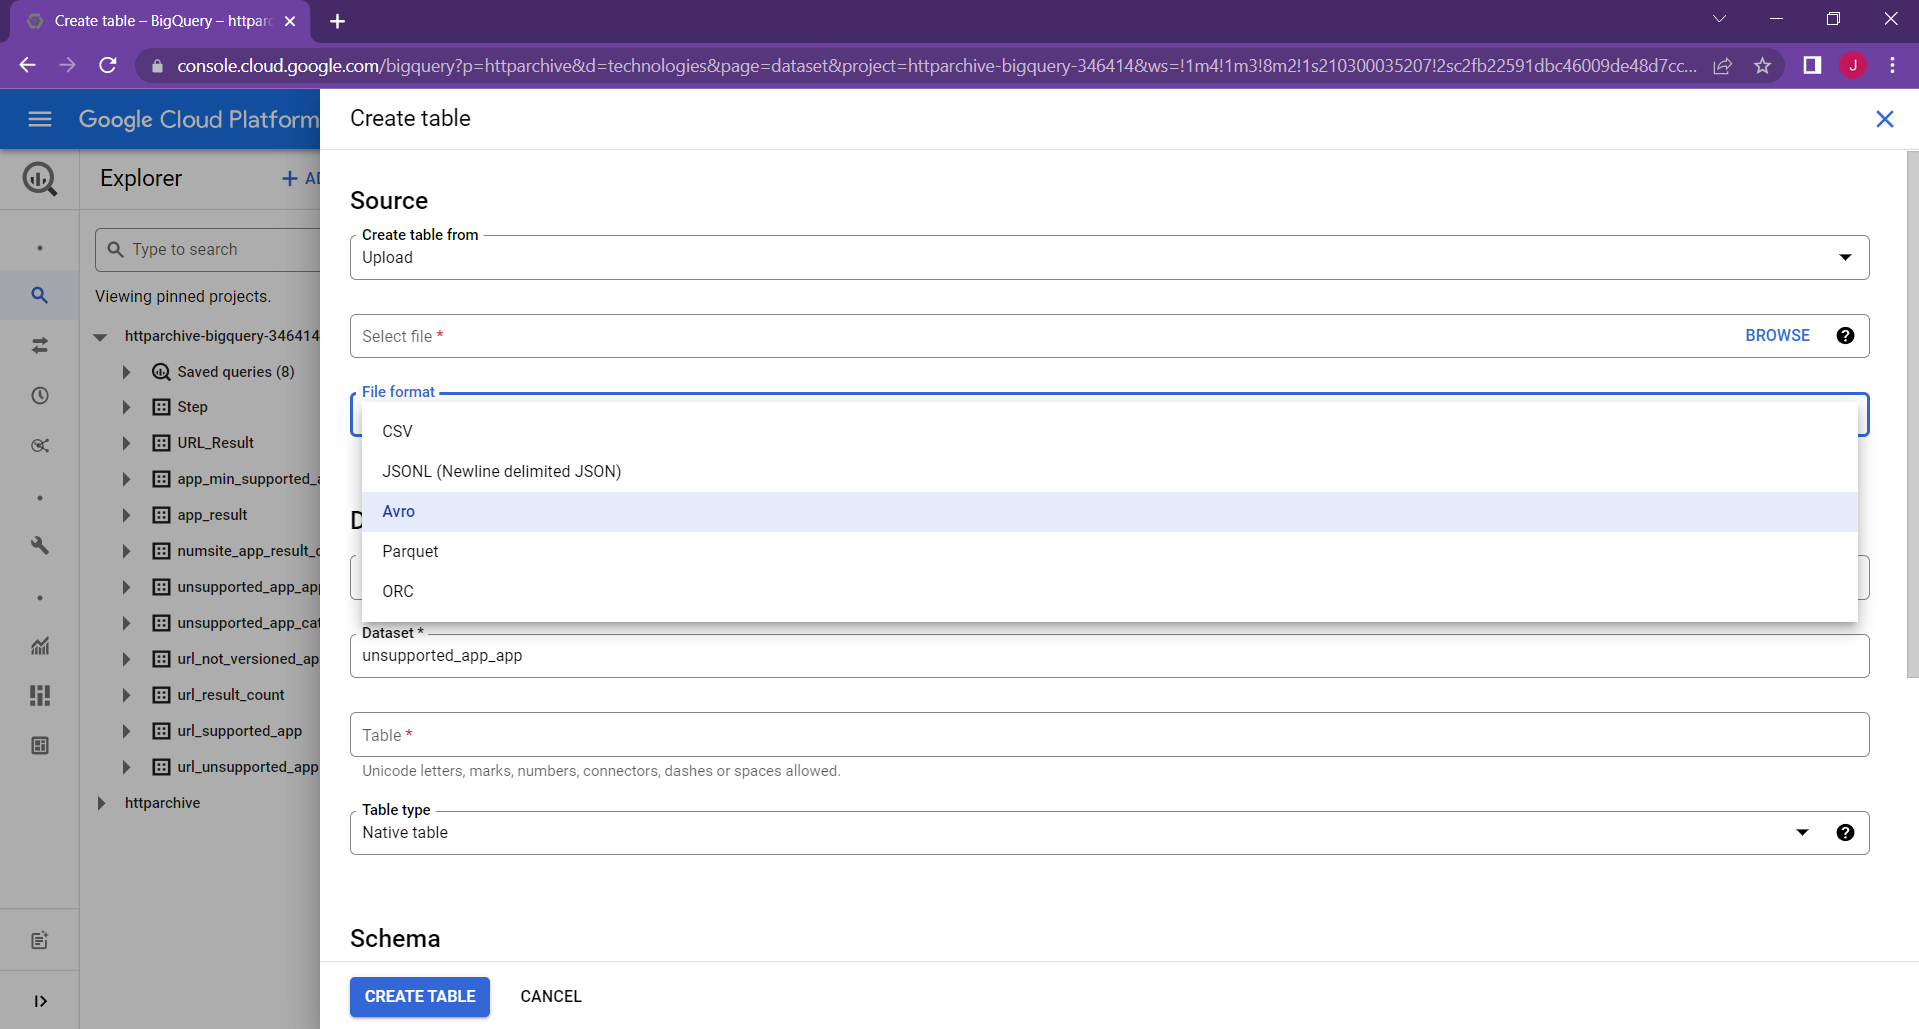
\includegraphics[scale=0.35]{Gambar/upload_step_3.png}  
		\caption{Pilih Lokasi dan Format File} 
		\label{fig:upload3}
	\end{figure}
\end{enumerate}


\section{\textit{Dataset} yang Digunakan pada HTTPArchive}
\textit{Dataset} pada HTTPArchive yang digunakan pada skripsi ini adalah sebagai berikut:
\begin{enumerate}
	\item technologies
	Pada tabel \textit{technologies} terdapat beberapa kolom seperti url, category, app, dan info. Url adalah alamat dari sebuah \textit{website}. Contoh dari \textit{dataset} dapat dilihat pada tabel \ref{table:ct_tech_desktop} 
	\begin{table}[H]
		\centering
		\begin{tabular}{|l|l|p{3cm}|p{3cm}|l|}
			\hline
			\textbf{Row} & \textbf{url} & \textbf{category} & app & info\\
			\hline
			1 & https://www.3-king.com/ & Analytics & Google Analytics & \\
			\hline
			2 & https://www.fleabites.net/ & Miscellaneous & Twitter Emoji (Twemoji) & \\
			\hline
			3 & http://www.elcarnicero.cl/ & Widgets & OWL Carousel & \\
			\hline
			4 & https://thankyou.ws/ & Analytics & Google Analytics & \\
			\hline
			5 & https://rogerwaters.com/ & Reverse proxies & Nginx & \\
			\hline
			6 & http://www.palaciodaslampadas.com.br/ & JavaScript libraries & jQuery & 2.1.1\\
			\hline
			7 & https://copenhagencamping.dk/ & CMS & WordPress & \\
			\hline
			8 & https://eachat.ma/ & Ecommerce & WooCommerce & 4.3.0\\
			\hline
			9 & https://advokat-bondarchuk.ru/ & Blogs & WordPress & \\
			\hline
			10 & https://passport.rsl.ru/ & JavaScript libraries & jQuery & 1.7.1\\
			\hline
		\end{tabular}
		\caption{Technologies Desktop Data Sample}
		\label{table:ct_tech_desktop}
	\end{table}
\end{enumerate}

\section{Langkah-Langkah Query Yang Dilakukan}
\label{langkah_query}
Pada section ini dijelaskan tentang langkah-langkah \textit{query} yang dilakukan dalam memperoleh data. Data yang diambil adalah data percobaan sebanyak 10 data. Data yang diambil merupakan \textit{dataset} dari tabel \textit{technologies} 2020$\_$08$\_$01:

\subsection{Mengumpulkan Daftar Website}
Langkah pertama yang dilakukan yaitu mengumpulkan \textit{website}. \textit{Website} yang dicari tidak berdasarkan \textit{rank} karena tidak tersedia pada \textit{dataset} tersebut. \textit{Query} yang digunakan untuk mengumpulkan daftar \textit{website} dapat dilihat pada Gambar \ref{lst:listwebsite10}.
\begin{lstlisting}[caption={Mencari Daftar \textit{Website} Limit 10}, label={lst:listwebsite10}]
SELECT 
	url
FROM 
	`httparchive.technologies.2020_08_01_*`
GROUP BY 
	url
LIMIT 10
\end{lstlisting}

Pada \textit{query} diatas dilakukan pemilihan pada kolom url dengan menggunakan perintah SELECT dari project httparchive dataset \textit{technologies} tabel 2020\_08\_01\_* dengan menggunakan perintah FROM. Mengelompokan pada kolom url yang dilakukan dengan menggunakan perintah GROUP BY sehingga tidak ada nama url yang sama. Kolom dibatasi sebanyak 10 baris dengan menggunakan perintah LIMIT. Sepuluh contoh hasil keluaran dari \textit{query} diatas dapat dilihat pada Tabel \ref{table:contoh_langkah1}:

\begin{table}[H]
\centering
\begin{tabular}{|l|l|}
	\hline
	\textbf{Row} & \textbf{url}\\
	\hline
	1 & https://www.theinsider.life/\\
	\hline
	2 & http://www.mtctutorials.com/ \\
	\hline
	3 & https://noticias24horases.com.br/\\
	\hline
	4 & https://www.tonyburke.com.au/ \\
	\hline
	5 & http://www.bakedbyjoanna.com/\\
	\hline
	6 & https://stuftburgerbar.com/\\
	\hline
	7 & https://www.skagitpowersports.com/\\
	\hline
	8 & http://www.arazatimaderas.com/ \\
	\hline
	9 & https://oasisexc.com/\\
	\hline
	10 & https://www.captainslanding.com/\\
	\hline
\end{tabular}
\caption{Hasil Pengumpulan Daftar Website}
\label{table:contoh_langkah1}
\end{table}

\subsection{Mencari Aplikasi Yang Digunakan \textit{Website}}
Setiap \textit{website} dicari aplikasi apa saja yang digunakan dalam pembangunan \textit{website} tersebut dari aplikasi yang dipakainya. \textit{Query} yang digunakan dapat dilihat pada Gambar \ref{lst:webapp10}.
\begin{lstlisting}[caption={Mencari Aplikasi yang Digunakan Website Limit 10}, label={lst:webapp10}]
SELECT DISTINCT 
	url, app
FROM 
	`httparchive.technologies.2020_08_01_*`
ORDER BY 
	url asc
LIMIT 10
\end{lstlisting}

Pada \textit{query} diatas dilakukan pemilihan pada kolom url dan app dengan menggunakan perintah SELECT dari \textit{project} httparchive \textit{dataset} \textit{technologies} tabel 2020\_08\_01\_* dengan menggunakan perintah FROM. Kolom diurutkan berdasarkan url secara \textit{ascending}. Kolom dibatasi sebanyak 10 baris dengan menggunakan perintah LIMIT. Sepuluh contoh hasil keluaran dari \textit{query} diatas dapat dilihat pada Tabel \ref{table:contoh_langkah2}:

\begin{table}[H]
\centering
\begin{tabular}{|l|l|l|}
	\hline
	\textbf{Row} & \textbf{url} & \textbf{app}\\
	\hline
	1 & http://0-1.ru/ & Liveinternet\\
	\hline
	2 & http://0-1.ru/ & Yandex.Metrika\\
	\hline
	3 & http://0-1.ru/ & IIS\\
	\hline
	4 & http://0-1.ru/ & Microsoft ASP.NET\\
	\hline
	5 & http://0-1.ru/ & YouTube\\
	\hline
	6 & http://0-1.ru/ & Windows Server\\
	\hline
	7 & 	
	http://0-10-10.cocolog-nifty.com/  & 	
	Nginx \\
	\hline
	8 & 	
	http://0-10-10.cocolog-nifty.com/  & Twitter\\
	\hline
	9 & 	
	http://0-10-10.cocolog-nifty.com/  & jQuery\\
	\hline
	10 & 	
	http://0-10-10.cocolog-nifty.com/  & Osano\\
	\hline
\end{tabular}
\caption{Contoh Aplikasi Yang Digunakan Website}
\label{table:contoh_langkah2}
\end{table}

\subsection{Mengelompokkan Berdasarkan Nama Semua Aplikasi Yang Dipakai}
Pengelompokan aplikasi dapat dilakukan dengan menggunakan \textit{query}. \textit{Query} yang digunakan dapat dilihat pada Gambar \ref{lst:groupapp10}.
\begin{lstlisting}[caption={Mengelompokan Semua Aplikasi yang Dipakai}, label={lst:groupapp10}]
SELECT 
	tabelName.app, num.num_sites , versioned.versioned_count , unversioned.unversioned_count
FROM 
(SELECT DISTINCT 
	app
FROM 
	`httparchive.technologies.2020_08_01_*` ) tabelName

LEFT JOIN 

(SELECT 
	tabel1.app, count(app) AS versioned_count
FROM 
	`httparchive.technologies.2020_08_01_*` AS tabel1
WHERE 
	tabel1.app!="" AND tabel1.info != "" 
GROUP BY 
	tabel1.app) AS versioned

ON(versioned.app = tabelName.app)

LEFT JOIN

(SELECT 
	tabel2.app, count(app) AS unversioned_count
FROM 
	`httparchive.technologies.2020_08_01_*` AS tabel2
WHERE 
	tabel2.app!="" AND tabel2.info = "" 
GROUP BY 
	tabel2.app) AS unversioned

ON (unversioned.app = tabelName.app)

LEFT JOIN 

(SELECT 
	app, count(url) AS num_sites
FROM 
	`httparchive.technologies.2020_08_01_*`
GROUP BY 
	app) AS num

ON (tabelName.app = num.app)
LIMIT 10
\end{lstlisting}

Pada \textit{query} diatas dibuat beberapa tabel baru yang bersifat sementara. Pada baris ke 3 dan 4, \textit{query} mengembalikan tabel yang berisi semua app yang ada pada tabel menggunakan perintah SELECT dan menggunakan DISTINCT agar app yang ditampilkan hanya keluar satu kali. Data diambil dari \textit{project} httparchive \textit{dataset} \textit{technologies} tabel 2020\_08\_01\_* dengan menggunakan perintah FROM. Kemudian pada baris ke 8 sampai 11, \textit{query} mengembalikan tabel yang berisi app dan jumlah app yang memiliki info tidak kosong atau memiliki informasi versi. Pada baris 17 sampai 22, \textit{query} mengembalikan tabel yang berisi app dan jumlah app yang tidak memiliki informasi versi. Pada baris 26 sampai dengan baris 28, \textit{query} mengembalikan tabel app, jumlah url yang menggunakan app tersebut. Kemudian semua tabel tersebut digabungkan dengan perintah LEFT JOIN. Kemudian dengan menggunakan perintah SELECT, dipanggil beberapa variabel dari setiap kolom dari setiap tabel. Kolom yang diambil berupa: app, jumlah situs yang dipakai aplikasi (num\_sites), jumlah aplikasi yang memiliki versi (versioned\_count), dan jumlah aplikasi yang tidak memiliki versi (unversioned\_count). Kolom dibatasi sebanyak 10 baris dengan menggunakan perintah LIMIT. Sepuluh contoh hasil keluaran dari \textit{query} diatas dapat dilihat pada Tabel \ref{table:contoh_langkah3}:

\begin{table}[H]
\centering
\begin{tabular}{|l|l|r|r|r|}
	\hline
	\textbf{Row} & \textbf{app} & \textbf{num\_sites} & \textbf{versioned\_count} & \textbf{unversioned\_count}\\
	\hline
	1 & jQuery & 10.003.030 & 9.979.001 & 24.029\\
	\hline
	2 & Apache & 4.067.380 & 1.118.200 & 2.949.180\\
	\hline
	3 & PHP & 5.977.790 & 2.522.620 & 3.455.170\\
	\hline
	4 & MySQL & 4.047.343 & null & 4.047.343\\
	\hline
	5 & Microsoft SharePoint & 14.419 & 11.402 & 3.017\\
	\hline
	6 & YouTube & 1.028.360& null & 1.028.360\\
	\hline
	7 & Microsoft ASP.NET & 865.276 & 407.366 & 457.910\\
	\hline
	8 & Google Code Prettify & 32.171 & null & 32.171\\
	\hline
	9 & Typekit & 253.890 & 253.203 & 687\\
	\hline
	10 & Slick & 759.805 & 66.249 & 693.556\\
	\hline
\end{tabular}
\caption{Hasil Pengelompokan Aplikasi Beserta Jumlah \textit{Versioned} Dan \textit{Unversioned}}
\label{table:contoh_langkah3}
\end{table}

Pada \cite{pascal}, jumlah data yang digunakan lebih sedikit sehingga jumlah keseluruhan data juga berbeda. Terdapat beberapa aplikasi yang sama sehingga dapat dibandingkan datanya. Tabel pada \cite{pascal} dapat dilihat pada Tabel \ref{table:contoh_tabel_paper}: 

\begin{table}[H]
\centering
\begin{tabular}{|p{1cm}|wr{0.1\linewidth}|wr{0.11\linewidth}|wr{0.13\linewidth}|wr{0.1\linewidth}|p{3 cm}|wr{0.12\linewidth}|}
	\hline
	\textbf{Name} & \textbf{num-sites} & \multirow{2}{0.11\linewidth}{\textbf{avg-confidence}} & \multirow{2}{0.13\linewidth}{\textbf{num-unversioned}} & \multirow{2}{0.1\linewidth}{\textbf{num-versioned}} & \textbf{website} & \multirow{3}{0.12\linewidth}{\textbf{num-supported-version}}\\
	&  &  &  &  &  &  \\
	&  &  &  &  &  &  \\
	\hline
	jQuery & 1.011 & 99.70 & 14 & 997 & https://jquery.com & >=3 \\
	\hline
	Boot strap & 340 & 99.30 & 88 & 342 & https://getboot strap.com & >=4 \\
	\hline
	JQuery Migrate & 298 & 99.66 & 31 & 267 & https://github.com /jquery/jquery-migrate & ?\\
	\hline
	PHP & 591 & 99.83 & 348 & 245 & https://www.php .net & >=7.2 \\
	\hline
	Font Awesome & 400 & 99.50 & 160 & 240 & https://fontaweso me.com & >=5 \\
	\hline
	JQuery UI & 176 & 99.43 & 7 & 169 & https://jqueryui .com & ? \\
	\hline
	Word Press & 346 & 100.00 & 181 & 165 & https://wordpress .org & >=5.4.2 \\
	\hline
	Under score.js & 124 & 24.19 & 2 & 122 & https://underscore js.org & ? \\
	\hline
	Lodash & 125 & 59.20 & 3 & 122 & https://lodash.com & ? \\
	\hline
	
	
\end{tabular}
\caption{Tabel Sepuluh Data Aplikasi Pada \cite{pascal}}
\label{table:contoh_tabel_paper}
\end{table}

\subsection{Mencari Data Tentang Versi Aplikasi Yang Masih Didukung}
Sebelum menentukan suatu aplikasi usang atau tidak, kita harus mencari versi dari setiap aplikasi secara manual. Versi setiap aplikasi dapat dilihat di \textit{official documentation} dari setiap aplikasi. Hasil pencarian dari aplikasi yang masih didukung dapat dilihat pada Tabel \ref{lamp:A}. 

\subsection{Melakukan Perbandingan Antara Versi Aplikasi Yang Masih Dipakai Sekarang Dengan Versi Aplikasi Yang Masih Didukung} \label{version_compare}
Setelah mendapatkan data versi minimal dari setiap aplikasi, data tersebut dibandingkan dengan versi aplikasi yang dipakai \textit{url}. \textit{Supported} adalah versi aplikasi dari yang dipakai \textit{url} masih mendukung atau diatas atau sama dengan versi yang didukung di dokumen. \textit{unsupported} adalah versi aplikasi dari yang dipakai url sudah tidak mendukung atau dibawah versi yang didukung didokumen. \textit{not\_versioned} adalah versi aplikasi dari url tidak ditampilkan. \textit{non\_conclusive} adalah versi aplikasi tidak dapat ditentukan. \textit{Query} yang digunakan dapat dilihat pada Gambar \ref{lst:normalize}, Gambar \ref{lst:compare}, Gambar \ref{lst:groupingversion}, dan Gambar \ref{lst:showitem}
\begin{lstlisting}[caption={Normalize Semantic Version}, label={lst:normalize}]
CREATE TEMP FUNCTION normaizedSemanticVersion(semanticVersion STRING) 
AS ((
SELECT STRING_AGG(
IF(isDigit, REPEAT('0', 100 - LENGTH(chars)) || chars, chars) ORDER BY grp 
)
FROM (
SELECT 
	grp, isDigit, STRING_AGG(char, '' ORDER BY OFFSET) chars,
FROM (
SELECT 
	OFFSET, char, isDigit,
COUNTIF(NOT isDigit) OVER(ORDER BY OFFSET) AS grp
FROM 
	UNNEST(SPLIT(semanticVersion, '')) AS char WITH OFFSET, 
UNNEST([char IN ('1','2','3','4','5','6','7','8','9','0')]) isDigit
)
GROUP BY 
	grp, isDigit
)));
\end{lstlisting}

\begin{lstlisting}[caption={Compare Semantic Version}, label={lst:compare}]
CREATE TEMP FUNCTION compareSemanticVersions(
normSemanticVersion1 STRING, 
normSemanticVersion2 STRING) 
AS ((
SELECT CASE 
WHEN info < min_supported 
	THEN 'UNSUPPORTED'
ELSE 
	'SUPPORTED'
END
FROM UNNEST([STRUCT(
normaizedSemanticVersion(normSemanticVersion1) AS info, 
normaizedSemanticVersion(normSemanticVersion2) AS min_supported
)])
));
	\end{lstlisting}

\begin{lstlisting}[caption={Membuat Tabel Sementara untuk Grouping Version}, label={lst:groupingversion}]
WITH test AS (
SELECT 
	url, category, app, if (array_length(split(info , ".")) > 2, split(info , ".")[offset(0)] || "." || split(info , ".")[offset(1)], info)  as info, min_supported	
FROM
	`httparchive-bigquery-346414.app_min_supported_and_info.app_min_supported_and_info`
WHERE 
	info != "\\"
GROUP BY 
	url, category, app, info, min_supported
)
	\end{lstlisting}

\begin{lstlisting}[caption={Menampilkan Hasil dari Perbandingan Versi}, label={lst:showitem}]
SELECT 
	url, category, app, info, min_supported, if(info = '', "NOT VERSIONED",if(min_supported = '?','NON CONCLUSIVE',compareSemanticVersions(info, min_supported)) ) as  result
FROM 
	test 
ORDER BY 
	url
\end{lstlisting}
Pada awalnya dibuat sebuah fungsi dengan nama \textit{normaizedSemanticVersion(semanticVersion STRING)}, dan \textit{compareSemanticVersions(normSemanticVersion1 STRING, normSemanticVersion2 STRING)}. Kemudian pada baris 29 sampai dengan 33, dibuat sebuah tabel sementara untuk membuat \textit{group} versi aplikasi yang dipisahkan berdasarkan titik.


Setelah melakukan perbandingan versi tersebut, data diteliti dan berikut ini adalah hasil sepuluh data yang dapat dilihat pada Tabel \ref{table:contoh_langkah5.1}. Data diambil berdasarkan banyak aplikasi yang dipakai oleh url tertentu. 
\begin{table}[H]
\centering
\begin{tabular}{|l|r|r|r|r|}
	\hline
	\textbf{url} & \textbf{supported} & \textbf{unsupported} & \textbf{not\_versioned} & \textbf{non\_conclusive}\\
	\hline
	authservice.pegipegi.com & 0 & 9 & 224 & 2\\
	\hline
	serviceauth.pegipegi.com & 0 & 13 & 220 & 2\\
	\hline
	mcatselfprep.com &0 & 14 & 52 & 8\\
	\hline
	perpetua.it & 0 & 14 & 50 & 12\\
	\hline
	sulava.com & 0 & 10 & 59 & 10\\
	\hline
	
	theraceclub.com & 2 & 12 & 48 & 16\\
	\hline
	
	jobs.discover.com & 4 & 8 & 58 & 8\\
	\hline
	
	dickssportinggoods.jobs & 4 & 8 & 56 & 8 \\
	\hline
	careers.symphonytalent.com & 4 & 8 & 56 & 8 \\
	\hline
	
	jobs.cedarfair.com & 4 & 8 & 52 & 12\\
	\hline
\end{tabular}
\caption{Hasil Perbandingan Aplikasi Berdasarkan url}
\label{table:contoh_langkah5.1}
\end{table}

%Data juga dikelompokkan berdasarkan \textit{category} yang memiliki aplikasi yang \textit{unsupported}. Kemudian \textit{category} tersebut dihitung kembali dan dikelompokkan berdasarkan jumlah aplikasi yang \textit{unsupport}-nya. Hasil dapat dilihat pada tabel \ref{table:contoh_langkah5.2}.
%\begin{table}[H]
%\centering
%\begin{tabular}{|r|r|r|r|r|}
%	\hline
%	\textbf{n=0} & \textbf{n=1} & \textbf{n=2} & \textbf{n=3} & \textbf{n>=4}\\
%	\hline
%	2 & 1 & 0 & 0 & 58\\
%	\hline
%\end{tabular}
%\caption{Jumlah Category Dengan Aplikasi Unsupported}
%\label{table:contoh_langkah5.2}
%\end{table}

Data juga dibandingkan berdasarkan aplikasi tertentu. Data yang dihasilkan adalah \textit{num\_sites} atau jumlah url yang menggunakan aplikasi tertentu, app, \textit{supported} atau aplikasi yang masih didukung, \textit{unsupported} atau aplikasi yang sudah tidak didukung, \textit{not\_versioned} atau aplikasi yang tidak diberi informasi versi, dan \textit{non\_conclusive} atau versi aplikasi tidak dapat ditentukan. Hasil dari data dapat dilihat pada Tabel \ref{table:contoh_langkah5.3}.
\begin{adjustwidth}{-2.5 cm}{-2.5 cm}\centering\begin{threeparttable}[!htb]
	\begin{tabular}{|r|l|r|r|r|r|}
		\hline
		\textbf{num\_sites} & \textbf{app} & \textbf{supported} & \textbf{unsupported} & \textbf{not\_versioned} & \textbf{non\_conclusive}\\
		\hline
		10.003.030 &jQuery &1.604.830 &8.374.171 &24.029 &0 \\
		\hline
		8.190.668 &Google Analytics &0 &0 &8.190.668 &0 \\
		\hline
		7.494.642 &WordPress &350 &4.891.016 &2.603.276 &0 \\
		\hline
		7.230.612 &Nginx &652 &1.789.692 &5.440.268 &0 \\
		\hline
		5.977.790 &PHP &167.095 &2.355.525 &3.455.170 &0 \\
		\hline
		5.481.111 &Google Font API &0 &0 &5.481.111 &0 \\
		\hline
		4.529.823 &Google Tag Manager &0 &0 &4.529.823 &0 \\
		\hline
		4.067.380 &Apache &764.690 &353.510 &2.949.180 &0 \\
		\hline
		4.047.343 &MySQL &0 &0 &4.047.343 &0 \\
		\hline
	\end{tabular}
	\caption{Hasil Perbandingan Aplikasi}
	\label{table:contoh_langkah5.3}
\end{threeparttable}\end{adjustwidth}


\section{Hasil \textit{Sample} Data Apache}
Diambil satu data \textit{sample} dengan aplikasi dan informasi versinya. Data \textit{sample} tersebut merupakan data Apache. Data dapat dilihat pada Gambar \ref{fig:data_sample_res}.
\begin{figure}[H]
\centering  
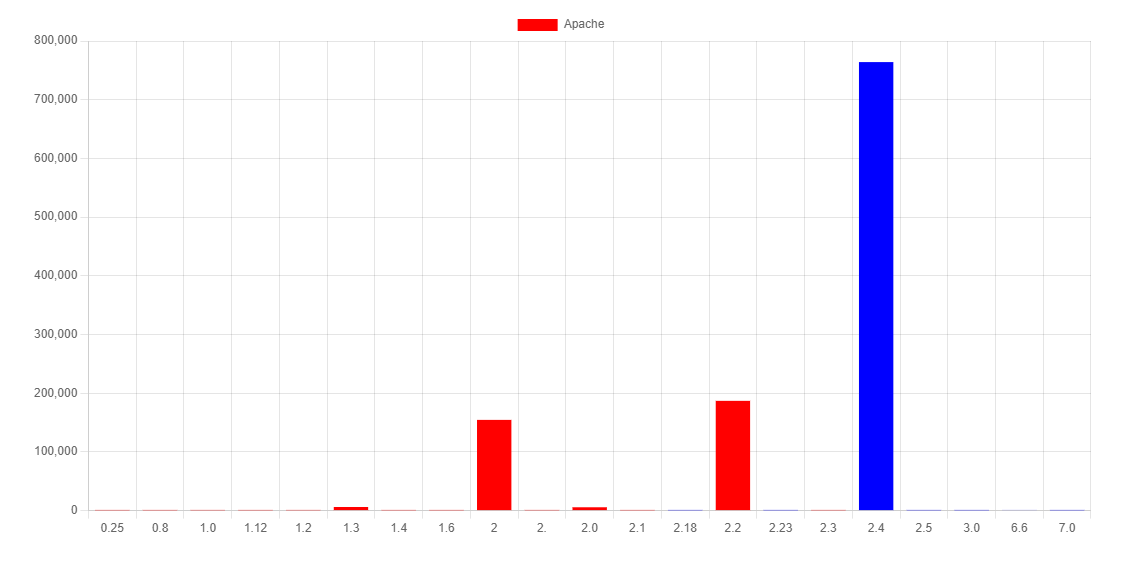
\includegraphics[scale=0.7]{Gambar/apache.PNG}  
\caption{Data Sample Jumlah Aplikasi Dengan Versi yang Dipakai} 
\label{fig:data_sample_res} 
\end{figure}
Pada data \ref{fig:data_sample_res} terdapat bagian bawah yang menunjukkan informasi versi dari aplikasi dan bagian kiri merupakan jumlah url yang menggunakan aplikasi. \textit{Chart} yang berwarna merah adalah \textit{chart} yang menunjukkan versi aplikasi tersebut sudah tidak didukung. \textit{Chart} yang berwarna biru menunjukkan versi aplikasi tersebut masih didukung.